% Monograph LaTeX Template for UFSC based on:
%
% 1. https://github.com/royertiago/tcc
% 2. http://portal.bu.ufsc.br/normalizacao/
% 3. https://github.com/AdrianoRuseler/abntex2-ufsc
%
% When the bibliography includes a cyclic reference to another bibliography,
% you need to run `pdfTeX` 5 times on the following order:
% 1. `pdfTeX`,
% 2. `biber`,
% 3. `pdfTeX`
% 4. `pdfTeX`
% 5. `pdfTeX`
% 6. `biber`
% 7. `pdfTeX`


% Allows you to write your thesis both in English and Portuguese
% https://tex.stackexchange.com/questions/5076/is-it-possible-to-keep-my-translation-together-with-original-text
\newif\ifenglish\englishfalse

% Uncomment the line `\englishtrue` to set the document default language to 
% English
% \englishtrue

% https://tex.stackexchange.com/questions/131002/how-to-expand-ifthenelse-so-that-it-can-be-used-in-parshape
\newcommand{\lang}[2]{\ifenglish#1\else#2\fi}

% https://tex.stackexchange.com/questions/385895/how-to-make-passoptionstopackage-add-the-option-as-the-last
\ifenglish
    \PassOptionsToPackage{brazil,main=english,spanish}{babel}
\else
    \PassOptionsToPackage{main=brazil,english,spanish}{babel}
\fi

% Simple alias for English and Portuguese words
\newcommand{\brazilword}[1]{\foreignlanguage{brazil}{#1}}
\newcommand{\englishword}[1]{\foreignlanguage{english}{#1}}

% Allow you to write `Evandro's house` in latex as `Evandro\s house` 
% instead of `Evandro\textquotesingle{}s house`
% https://tex.stackexchange.com/questions/31091/space-after-latex-commands
\newcommand{\s}[0]{\textquotesingle{}s\xspace}
\newcommand{\q}[0]{\textquotesingle{}\xspace}

% Uncomment the following line if you want to use other biblatex settings
% \PassOptionsToPackage{style=numeric,repeatfields=true,backend=biber,backref=true,citecounter=true}{biblatex}

% Disable the empty pages automatically put by memoir class, except the ones by \cleardoublepage
% \PassOptionsToClass{openany}{memoir}

% Fixes several `abntex2` class problems
\input{setup/setup.tex}

% The UFSC font size is 10.5, but memoir embedded by `abntex2` only accepts 10 and 11pt.
% However, problem will be fixed the `ufscthesisx` package.
\documentclass[
% 10pt,          % Padrão UFSC para versão final
% a5paper,       % Padrão UFSC para versão final
12pt,          % Pode usar tamanho 12pt para defesa
a4paper,       % Pode usar a4 para defesa
% twoside,       % Impressão nos dois lados da folha
chapter=TITLE, % Título de capítulos em caixa alta
section=TITLE, % Título de seções em caixa alta
]{abntex2}

% Set the page size to be A4 as opposed to the default US Letter
% \usepackage[a4paper, margin=2cm]{geometry}

% Load the UFSC thesis package
\usepackage{setup/ufscthesisx}

% Load the symbols defined in symbols.sty 
\usepackage{symbols} 

% Load extra commands for tables, lists, summaries, etc.
\input{setup/utilities.tex}

% Load tikz and tikz libraries
\usepackage{tikz}
\usetikzlibrary{arrows, decorations, backgrounds, positioning, shapes.misc,
                calc}

% create some tikz styles
\tikzstyle{pickup} = [rectangle,minimum size=6mm]
\tikzstyle{delivery} = [circle,minimum size=8mm]
\tikzstyle{request1}=[draw=green!50,fill=green!20]
\tikzstyle{request2}=[draw=blue!50,fill=blue!20]
\tikzstyle{garage}=[circle,minimum size=6mm, draw=black!50,fill=black!5]
\tikzstyle{pre}=[<-,>=stealth',semithick]
\tikzstyle{post}=[->,>=stealth',semithick]
\tikzstyle{duo}=[<->,>=stealth',semithick]
\tikzstyle{pickuptw}=[rectangle, minimum width=10mm, minimum height=4mm]
\tikzstyle{deliverytw}=[rounded rectangle, minimum width=20mm, 
                       minimum height=4mm]
\tikzstyle{timeline}=[|-|]



% % Utilize o arquivo aftertext/references.bib para incluir sua bibliografia.
\addbibresource{aftertext/references.bib}

\autor{\brazilword{Renan Artur Lopes Eccel}}
\titulo{\lang
  {Dynamic Pickup and Delivery Problems \\ with Time Windows}
  {Problemas Dinâmicos de Coleta \\ e Entrega com Janelas de Tempo}}

\subtitulo{\lang{Benchmark Instances}{Análise de Instâncias de Benchmark}}

% Siglas para grau de formação Dr./Dra., Me./Ma, Bel. Bela. 
% (inglês: PhD., MSc., Bs.)
\orientador[\lang{Supervisor}{Orientador}]
           {\brazilword{Prof. Rodrigo Castelan Carlson}, 
           \lang{Phd.}{Dr.} \lang{}{}}

% Preencher com o nome do Coordenador de TCCs/Teses do seu curso
\coordenador[\lang{Coordinator}{Coordenador}]
            {\brazilword{Prof. Werner Kraus Jr.}, 
            \lang{Phd.}{Dr.} \lang{}{}}

% Local da sua defesa
\local{\brazilword{Florianópolis}}

% Ano da sua defesa
\ano{2019}
\biblioteca{\lang{University Library}{Biblioteca Universitária}}

% Sigla da sua instituição
\instituicaosigla{UFSC}
\instituicao{\lang{Federal University of}{Universidade Federal de} 
             \brazilword{Santa Catarina}}

% Preencha com Tese, Dissertação, Monografia ou Trabalho de 
% Conclusão de Curso, Bachelor's Thesis, etc
\tipotrabalho{\lang{Monograph}{Dissertação}}

% FIXME: Se houver Área de Concentração, descomente a linha abaixo
% \area{\lang{Concentration Area}{Área de Concentração}}

% Preencha com Doutor, Bacharel ou Mestrando
\formacao{\lang
    {Master in Automation and Systems Engineering}
    {Mestre em Engenharia de Automação e Sistemas}%
}
\programa{\lang
    {Postgraduate Program in Automation and Systems Engineering}
    {Programa de Pós-Graduação em Engenharia de Automação e Sistemas}%
}

% Preencha com Departamento de XXXXXX, Centro de XXXXXX
\centro{\lang
    {Department of Automation and Systems, Center of Technology}
    {Departamento de Automação e Sistemas, Centro Tecnológico}%
}

% Data da sua defesa
\data{\lang{28 of August of}{28 de agosto de} 2019}

% O preambulo deve conter tipo do trabalho, objetivo, nome da instituição 
% e a área de concentração.
\preambulo{\lang%
    {%
        \imprimirtipotrabalho~submitted to the \imprimirprograma~of
        \imprimirinstituicao~for degree acquirement in \imprimirformacao.%
    }{%
        \imprimirtipotrabalho~submetida ao \imprimirprograma~da
        \imprimirinstituicao~para a obtenção do título de \imprimirformacao.%
    }%
}

\palavraschaveufsc{palavraschaveingles}   {Routing}
\palavraschaveufsc{palavraschaveportugues}{Roteamento}

\palavraschaveufsc{palavraschaveingles}   {Dynamic}
\palavraschaveufsc{palavraschaveportugues}{Dinâmico}

\palavraschaveufsc{palavraschaveingles}   {Instance}
\palavraschaveufsc{palavraschaveportugues}{Instância}

\palavraschaveufsc{palavraschaveingles}   {Benchmark}
\palavraschaveufsc{palavraschaveportugues}{Benchmark}

\palavraschaveufsc{palavraschaveingles}   {PDPTW}
\palavraschaveufsc{palavraschaveportugues}{PDPTW}

\palavraschaveufsc{palavraschaveingles}   {DARP}
\palavraschaveufsc{palavraschaveportugues}{DARP}

% Altere o arquivo 'settings.tex' para incluir customizações de aparência 
% da sua tese
%----------------------------------------------------------------------------------------
%   File settings
%----------------------------------------------------------------------------------------

% Comment this, unless you are debugging pages' badness Underfull & Overflow
% https://tex.stackexchange.com/questions/115908/geometry-showframe-landscape
%
% What is the difference between \usepackage{showframe} and \usepackage[showframe]{geometry}?
% https://tex.stackexchange.com/questions/387077/what-is-the-difference-between-usepackageshowframe-and-usepackageshowframe
%
% How to do the memoir headings fix but not have my text going over the page bottom margins?
% https://tex.stackexchange.com/questions/387257/how-to-do-the-memoir-headings-fix-but-not-have-my-text-going-over-the-page-botto
%
% Print page margins of a document, for debugging bad boxes
% https://tex.stackexchange.com/questions/14508/print-page-margins-of-a-document
% \usepackage[showframe,pass]{geometry}


% To use the font Times New Roman, instead of the default LaTeX font
% more up-to-date than '\usepackage{mathptmx}'
% \usepackage{newtxtext}
% \usepackage{newtxmath}

% Novo list of (listings) para QUADROS usando newfloat
\usepackage{newfloat}
\makeatletter
%% we define a helper macro for adjusting lists of new floats to
%% accept a * behind them for not being shown in the TOC, like
%% the other list printing commands in memoir
% https://tex.stackexchange.com/questions/176418/remove-list-of-newfloat-from-toc
\newcommand{\AdjustForMemoir}[1]{%
  \csletcs{kept@listof#1}{listof#1}%
  \csdef{listof#1}{%
    \@ifstar
     {\csappto{newfloat@listof#1@hook}{\append@star}%
      \csuse{kept@listof#1}}%
     {\csuse{kept@listof#1}}%
  }
}
\def\append@star#1{#1*}
\makeatother
% \newcommand{\quadroname}{Quadro}
% \newcommand{\listofquadrosname}{Lista de Quadros}
\DeclareFloatingEnvironment[fileext=loq,placement={!hbtp},name=Quadro,within=chapter,listname=Lista de Quadros]{quadro}
\AdjustForMemoir{quadro}
\newlistentry{quadro}{loq}{0}



% Thesis settings
\newcommand{\brazilword}[1]{\foreignlanguage{brazil}{#1}}
\newcommand{\englishword}[1]{\foreignlanguage{english}{#1}}

\lang % Switch between english and brazil for big text blocks
{\includecomment{englishtext}\excludecomment{braziltext}}
{\includecomment{braziltext}\excludecomment{englishtext}}

% What is the difference between \def and \newcommand?
% https://tex.stackexchange.com/questions/655/what-is-the-difference-between-def-and-newcommand
\def\mytextpreliminarylistname{\lang{Brief Table of Contents}{Breve Sumário}}

% How to manually set where a word is split?
% https://tex.stackexchange.com/questions/182569/how-to-manually-set-where-a-word-is-split
\hyphenation{Ge-la-im}


% Patch the `abntex2` citacao environment
\xpatchcmd{\citacao}
{\list{}}
{\list{}{\topsep=0pt}}
{}
{\PackageWarning{ufscthesisx}{Citation \topsep is not patched. The 'citacao' environment must be
patched with 'topsep=0pt' but it failed. This is probably due an update on the main class 'abnTeX2',
therefore the \topsep patch must need to be updated accordingly}}

% Remove the colon appended to theses variables, allowing us to use other separators
\addto\captionsbrazil
{
    \renewcommand{\orientadorname}{Orientador}
    \renewcommand{\coorientadorname}{Coorientador}
}

% Create caption English translations as the sections headers
% https://tex.stackexchange.com/questions/8564/what-is-the-right-way-to-redefine-macros-defined-by-babel
\addto\captionsenglish
{
    %% adjusts names from abnTeX2
    \renewcommand{\folhaderostoname}{Title page}
    \renewcommand{\epigraphname}{Epigraph}
    \renewcommand{\dedicatorianame}{Dedication}
    \renewcommand{\errataname}{Errata sheet}
    \renewcommand{\agradecimentosname}{Acknowledgements}
    \renewcommand{\anexoname}{ANNEX}
    \renewcommand{\anexosname}{Annex}
    \renewcommand{\apendicename}{APPENDIX}
    \renewcommand{\apendicesname}{Appendix}
    \renewcommand{\orientadorname}{Supervisor}
    \renewcommand{\coorientadorname}{Co\hyp{}supervisor}
    \renewcommand{\folhadeaprovacaoname}{Approval}
    \renewcommand{\resumoname}{Abstract}
    \renewcommand{\listadesiglasname}{List of abbreviations and acronyms}
    \renewcommand{\listadesimbolosname}{List of symbols}
    \renewcommand{\fontename}{Source}
    \renewcommand{\notaname}{Note}
    %% adjusts names used by \autoref
    \renewcommand{\pageautorefname}{page}
    \renewcommand{\sectionautorefname}{section}
    \renewcommand{\subsectionautorefname}{subsection}
    \renewcommand{\subsubsectionautorefname}{subsubsection}
    \renewcommand{\paragraphautorefname}{subsubsubsection}
}

% Source Code Settings in Document
\makeatletter
\@ifpackageloaded{listings}
{
\ifenglish
    % These default values are already in English
\else
    % Listing -> Codigo fonte
    \renewcommand{\lstlistingname}{Código--fonte}

    % List of Listings -> Lista de códigos-fonte
    \renewcommand{\lstlistlistingname}{Lista de códigos--fonte}

    % Calculate the size of the header
    \calculatelisteningsheader
\fi
}{}
\makeatother


% Espaçamentos entre linhas e parágrafos
%
% ifpackageloaded question
% https://tex.stackexchange.com/questions/70212/ifpackageloaded-question
\makeatletter
\@ifclassloaded{memoir}
{
    % Estilo de capítulos, ver classe para maiores detalhes.Veja outros estilos em:
    % http://mirrors.ibiblio.org/CTAN/macros/latex/contrib/memoir/memman.pdf
    \chapterstyle{VZ14}
    \setlength\beforechapskip{0pt}
    \setlength\midchapskip{15pt}
    \setlength\afterchapskip{15pt}

    % O tamanho do parágrafo é dado por:
    \setlength{\parindent}{1.3cm}

    % Controle do espaçamento entre um parágrafo e outro. Tente também
    % \onelineskip
    \setlength{\parskip}{0.2cm}

    % Memoir: Warnings “The material used in the headers is too large” w/ accented titles
    % https://tex.stackexchange.com/questions/387293/how-to-change-the-page-layout-with-memoir
    \setheadfoot{30.0pt}{\footskip}
    \checkandfixthelayout
}{}
\makeatother


% Color settings across the document
\makeatletter
\@ifpackageloaded{xcolor}
{
    % RGB colors in absolute values from 0 to 255 by using `RGB` tag
    \definecolor{darkblue}{RGB}{26,13,178}

    % Definição de cores, RGB colors in percentage notation by using `rgb` tag
    \definecolor{mygreen}{rgb}{0,0.6,0}
    \definecolor{mygray}{rgb}{0.5,0.5,0.5}
    \definecolor{mymauve}{rgb}{0.58,0,0.82}

    % Configurações de aparência do PDF final
    \definecolor{figcolor}{rgb}{1,0.4,0}  % orange
    \definecolor{tabcolor}{rgb}{1,0.4,0}  % orange
    \definecolor{eqncolor}{rgb}{1,0.4,0}  % orange
    \definecolor{linkcolor}{rgb}{1,0.4,0} % orange
    \definecolor{citecolor}{rgb}{1,0.4,0} % orange
    \definecolor{seccolor}{rgb}{0,0,1}    % blue
    \definecolor{abscolor}{rgb}{0,0,1}    % blue
    \definecolor{titlecolor}{rgb}{0,0,1}  % blue
    \definecolor{biocolor}{rgb}{0,0,1}    % blue

    % Alterando o aspecto da cor azul
    \definecolor{blue}{RGB}{41,5,195}

    % Informações do PDF
    \@ifpackageloaded{hyperref}
    {
        \hypersetup
        {
            pdftitle={\@title},
            colorlinks=true, % false: boxed links; true: colored links
            linkcolor=darkblue, % color of internal links
            citecolor=darkgreen, % color of links to bibliography
            filecolor=black, % color of file links
            urlcolor=linkcolor,
            bookmarksdepth=4
        }
        \ifenglish
            \hypersetup
            {
                pdfauthor={Author},
                pdfsubject={Thesis' Abstract},
                pdfcreator={LaTeX with abnTeX2 for UFSC},
                pdfkeywords={abnt}{latex}{UFSC}{abntex2}{thesis},
            }
        \else
            \hypersetup
            {
                pdfauthor={Autores},
                pdfsubject={Resumo da tese},
                pdfcreator={LaTeX com abnTeX2 para UFSC},
                pdfkeywords={abnt}{latex}{UFSC}{abntex2}{tese},
            }
        \fi
    }
}{}
\makeatother


% Changing the font of the numbers in the ToC in the memoir class
% https://tex.stackexchange.com/questions/14314/changing-the-font-of-the-numbers-in-the-toc-in-the-memoir-class
\renewcommand{\cftpartfont}{\ABNTEXpartfont\color{ultramarine}}
\renewcommand{\cftpartpagefont}{\ABNTEXpartfont\color{black}}

\renewcommand{\cftchapterfont}{\ABNTEXchapterfont\color{ultramarine}}
\renewcommand{\cftchapterpagefont}{\ABNTEXchapterfont\color{black}}

\renewcommand{\cftsectionfont}{\ABNTEXsectionfont\color{ultramarine}}
\renewcommand{\cftsectionpagefont}{\ABNTEXsectionfont\color{black}}

\renewcommand{\cftsubsectionfont}{\ABNTEXsubsectionfont\color{ultramarine}}
\renewcommand{\cftsubsectionpagefont}{\ABNTEXsubsectionfont\color{black}}

\renewcommand{\cftsubsubsectionfont}{\ABNTEXsubsubsectionfont\color{ultramarine}}
\renewcommand{\cftsubsubsectionpagefont}{\ABNTEXsubsubsectionfont\color{black}}

\renewcommand{\cftparagraphfont}{\ABNTEXsubsubsubsectionfont\color{ultramarine}}
\renewcommand{\cftparagraphpagefont}{\ABNTEXsubsubsubsectionfont\color{black}}


% Backref package settings, pages with citations in bibliography
\makeatletter
\@ifpackageloaded{biblatex}
{
    \renewbibmacro*{pageref}
    {
        \iflistundef{pageref}
        {\printtext{\lang{\autocap{n}o citation in the text}{\autocap{n}enhuma citação no texto}.}}
        {%
            \printtext
            {%
                \ifnumgreater{\value{citecounter}}{1}
                    {\lang{\autocap{c}ited}{\autocap{c}itado} \arabic{citecounter} \lang{times}{vezes}}
                    {\lang{\autocap{c}ited}{\autocap{c}itado} \arabic{citecounter} \lang{time}{vez}}
            }%
            \setunit{\addspace}%
            \ifnumgreater{\value{pageref}}{1}
                {\bibstring{backrefpages}\ppspace}
                {\bibstring{backrefpage}\ppspace}%
            \printlist[pageref][-\value{listtotal}]{pageref}%
        }%
    }

    \DefineBibliographyStrings{brazil}
    {
        backrefpage  = {na página},
        backrefpages = {nas páginas},
    }

    \DefineBibliographyStrings{english}
    {
        backrefpage  = {on page},
        backrefpages = {on pages},
    }
}{}
\makeatother


% Memoir has another mechanism for the job: \cftsetindents{‹kind›}{indent}{numwidth}. Here kind is
% chapter, section, or whatever; the indent specifies the ‘margin’ before the entry starts; and the
% width is of the box into which the number is typeset (so needs to be wide enough for the largest
% number, with the necessary spacing to separate it from what comes after it in the line.
% http://www.tex.ac.uk/FAQ-tocloftwrong.html
%
% memoir: indentation of unnumbered sections in table of contents
% https://tex.stackexchange.com/questions/264668/memoir-indentation-of-unnumbered-sections-in-table-of-contents
%
% Memoir ToC: indent the second line by number+space width in the previous line OR set standard
% https://tex.stackexchange.com/questions/394227/memoir-toc-indent-the-second-line-by-numberspace

% `\cftlastnumwidth` and these `\cftsetindents` are defined by the abntex2 class saying they obey
% the `ABNTEXsumario-abnt-6027-2012`.
% \newlength{\cftlastnumwidth}

\setlength{\cftlastnumwidth}{\cftsubsubsectionnumwidth}
\addtolength{\cftlastnumwidth}{-1em}

% http://www.tex.ac.uk/FAQ-tocloftwrong.html
% Use \setlength\cftsectionnumwidth{4em} to override all these values
\cftsetindents{part}         {0em}{\cftlastnumwidth}
\cftsetindents{chapter}      {0em}{\cftlastnumwidth}
\cftsetindents{section}      {0em}{\cftlastnumwidth}
\cftsetindents{subsection}   {0em}{\cftlastnumwidth}
\cftsetindents{subsubsection}{0em}{\cftlastnumwidth}
\cftsetindents{paragraph}    {0em}{\cftlastnumwidth}
\cftsetindents{subparagraph} {0em}{\cftlastnumwidth}




% Allows you to use ~= instead of `\hyp{}`
% https://tex.stackexchange.com/questions/488008/how-to-create-an-alternative-to-shortcut-or-hyp
% \useshorthands{~}\defineshorthand{~=}{\hyp{}}

% When writing a large document, it is sometimes useful to work on selected 
% sections of the document to speed up compilation time: 
% https://en.wikibooks.org/wiki/TeX/includeonly
\newif\ifforcedinclude\forcedincludefalse

% \addtoincludeonly{beforetext/agradecimentos}
% \addtoincludeonly{beforetext/epigrafe}
% \addtoincludeonly{beforetext/fichacatalografica}
% \addtoincludeonly{beforetext/folhadeaprovacao}
% \addtoincludeonly{beforetext/resumos}
% \addtoincludeonly{beforetext/siglas}
% \addtoincludeonly{beforetext/simbolos}

% \addtoincludeonly{chapters/intro}
% \addtoincludeonly{chapters/chapter_1}
% \addtoincludeonly{chapters/chapter_2}
% \addtoincludeonly{chapters/chapter_3}
% \addtoincludeonly{chapters/chapter_4}
% \addtoincludeonly{chapters/conclusion}

% \addtoincludeonly{aftertext/anexo_a}
% \addtoincludeonly{aftertext/anexo_b}
% \addtoincludeonly{aftertext/apendice_a}

% Control whether the full document will be generated
% Note: It will also generate severals errors like the following, which can be ignored
%       Latexmk: Missing input file: 'chapters/test.aux'
%
% You can make latex stop generate these errors, if you generate a full version
% of the document, before uncommenting these lines.
%
% Uncomment these two lines, to only partially generate the document
% \doincludeonly
% \forcedincludetrue

\ifenglish
    \hypersetup
    {
        pdfauthor={Author},
        pdfsubject={Thesis' Abstract},
        pdfcreator={LaTeX with abnTeX2 for UFSC},
        pdfkeywords={abnt}{latex}{UFSC}{abntex2}{thesis},
    }
\else
    \hypersetup
    {
        pdfauthor={Autores},
        pdfsubject={Resumo da tese},
        pdfcreator={LaTeX com abnTeX2 para UFSC},
        pdfkeywords={abnt}{latex}{UFSC}{abntex2}{tese},
    }
\fi

\begin{document}

    % FIXME: Comment this after finishing the thesis, so you can start fixing the \flushbottom vs \raggedbottom
    % https://tex.stackexchange.com/questions/65355/flushbottom-vs-raggedbottom
    \raggedbottom

    % https://tex.stackexchange.com/questions/4705/double-space-between-sentences
    \frenchspacing

    % ELEMENTOS PRÉ-TEXTUAIS
    \input{beforetext/beforetext.tex}

    % ELEMENTOS TEXTUAIS
    \textual

    % Uncomment this to put a ←← | ← (Go To Top/Go Back) on each section header
    % \addGoToSummary
    \setlength\beforechapskip{50pt}
    \setlength\midchapskip{20pt}
    \setlength\afterchapskip{20pt}

    % PARTE
    % \ifforcedinclude\else\part{\lang{Research}{Pesquisa}}\fi
    % \label{sec:primeira_parte}

    % Introdução (sem numeração, mas presente no Sumário)
    \chapter{Introdução}\label{ch:introducao}

Problemas de roteamento dinâmico de veículos são objetos de pesquisa há cerca 
de três décadas \cite{psaraftis_dynamic_2015}.
Derivados de problemas de roteamento de veículos (VRP - \textit{Vehicle Routing 
Problem}) clássicos, como o problema \textit{dial-a-ride} (DARP -
\textit{Dial-A-Ride Problem}) e o problema de coleta e entrega com
janelas de tempo (PDPTW - \textit{Pickup and Delivery Problem with 
Time Windows}), os problemas dinâmicos buscam modelar casos em que um 
ou mais parâmetros do problema não são totalmente conhecidos 
\textit{a priori} e podem variar durante o período de operação. 

Dentre o grupo de problemas dinâmicos de roteamento veicular, o problema 
\textit{dial-a-ride} dinâmico (DDARP - \textit{Dynamic Dial-A-Ride Problem}) 
\cite{psaraftis_dynamic_1988} e o problema dinâmico de coleta e entrega com
janelas de tempo (DPDPTW - \textit{Dynamic Pickup and Delivery Problem with 
Time Windows}) \cite{dumas_1991} são de grande interesse para o 
desenvolvimento de novas tecnologias de transporte urbano. 
São esses os problemas que precisam ser solucionados quando precisa-se 
de um serviço de transporte compartilhado dinâmico (\textit{dynamic 
ride-sharing}) \cite{agatz_optimization_2012, 
alonso-gonzalez_potential_2018}, ou quando necessita-se 
fazer uma entrega imediata de encomendas \cite{pankratz_dynamic_2005}.
Atualmente, algumas empresas fornecem serviços desse tipo (Uber Pool, Uber
Eats, Rappi).
Entretanto, com o esperado avanço tecnológico na área de veículos
autônomos e a diversificação dos transportes públicos introduzida
principalmente por sistemas de mobilidade como um serviço (MaaS -
\textit{Mobility as a Service}), serão cada vez mais necessário algoritmos 
para a solução dos problemas DDARP e DPDPTW em menor tempo e proporcionando 
um melhor resultado \cite{fulton_three_2017}. 

Uma pesquisa científica na área de algoritmos para soluções de problemas 
desse tipo normalmente requer a montagem de uma simulação computacional,
já que testes empíricos são economicamente inviáveis para
esse tipo de pesquisa \cite{maciejewski_towards_2017}.
A ideia do uso de simulações é poder gerar resultados de eficiência e de 
tempo computacional dos métodos de solução dos problemas para, com isso, 
comparar diferentes algoritmos.

Entretanto, para que os resultados possam ser comparados entre artigos, sem a
necessidade de reproduzir resultados gerados anteriormente,
necessita-se que as simulações conduzidas usem os mesmos cenários de 
simulação.
Na área de VRP estáticos é comum a existência de conjuntos de cenários
canônicos extensivamente usados que facilitam a comparação entre 
algoritmos \cite{mendoza_vrp-rep:_2014}, chamados de
conjunto de instâncias de \textit{benchmark}.

Na área de roteamento dinâmico de veículos não existem instâncias
de \textit{benchmark} de referência que sejam amplamente usadas 
\cite{pillac_review_2013, maciejewski_towards_2017}. 
Isso faz com que a comparação entre algoritmos
propostos para resolver problemas como DPDPTW e DDARP seja difícil e custosa.

O objetivo deste artigo é compilar as informações disponíveis sobre as
instâncias de \textit{benchmark} de DDARPs e DPDPTWs que estejam acessíveis e
disponíveis para uso, com enfoque na forma com que são feitas a distribuição
dos pedidos ao longo do período de operação dos sistemas.
Também faz parte do escopo uma análise de duas medidas, urgência e 
grau de dinamismo, propostas por \citeonline{van_lon_measures_2016} que ajudam 
a identificar as características temporais das instâncias. 
Com isso, procura-se auxiliar o processo de busca e seleção de conjuntos de 
instâncias interessantes para uso em simulações e teste de novos algoritmos ou,
caso necessário, auxiliar a seleção de um método de geração de instâncias
dinâmicas adequado ao interesse de pesquisa.

% as linhas contidas entre \iffalse e \fi estão todas comentadas
% elas descrevem em mais detalhes a dificuldades de fazer uma pesquisa na área
% de algoritmos para problemas de roteamento, assim como algumas "dicas" para
% quem quer fazer o mesmo.
% Essa parte se encontra mal escrita, no entanto, pode ser interessante 
% adicionar algo dela na introdução 
\iffalse
Primeiramente, se faz necessário a utilização de um simulador para rodar
testes, já que testes empíricos são inviáveis para esse tipo de pesquisa.
Por muitos anos os pesquisadores optaram por implementar seus próprios 
simuladores e não disponibilizar o código de maneira aberta, isso fez com que a
comunidade perdesse uma grande oportunidade de cooperação.
Com um código de livre acesso outros pesquisadores possuem a possibilidade de
reutilizar o código, facilitando as implementações de pesquisas na área, além
de poder revisar, melhorar ou estender o código. 
Atualmente, apesar de não serem amplamente usados, já existem simuladores de 
problemas de roteamento dinâmico com código aberto disponíveis para livre uso
acadêmico (\cite{van_lon_rinsim:_2012}; \cite{mayer_open-source_2016};
\cite{maciejewski_towards_2017})

Após a escolha de um simulador já disponível ou a implementação de um novo, se
faz necessária a implementação do algoritmo a ser testado. 
É nessa etapa que o pesquisador aplica seus conhecimentos técnicos para a 
implementação do seu objeto de pesquisa.

Após essa implementação precisa-se então da comparação de performance entre
o novo algoritmo e os algoritmos propostos anteriormente.
Para isso existem dois métodos.

Um deles é o pesquisador implementar os algoritmos com base na descrição dada 
nos artigos publicados, tarefa que, normalmente, toma bastante tempo do 
pesquisador e não agrega nenhum valor.
Atualmente, já existem pesquisadores que montam seus experimentos e deixam
disponíveis para acesso, replicação e utilização (\cite{van_lon_towards_2015};
\cite{van_lon_measures_2016}; \cite{van_lon_when_2017}).

Uma outra forma de comparação de algoritmos é possível quando os experimentos
são baseados em cenários cujos dados estão disponíveis para todos e
que já foram utilizados para testes em algoritmos de outros artigos.
A esse conjunto de dados se dá o nome de conjunto de instâncias de
\textit{benchmark}.
Portanto, quando usado um conjunto de instâncias de \textit{benchmark}, os
resultados expostos nos artigos podem ser comparados diretamente, sem a
necessidade de replicação dos experimentos.
Entretanto, na área de roteamento dinâmico de veículos não existem instâncias
de \textit{benchmark} de referência que sejam amplamente usadas
\cite{pillac_review_2013}

O objetivo deste artigo é compilar as informações disponíveis sobre as
instâncias de \textit{benchmark} de DDARPs e DPDPTWs que estejam acessíveis e
disponíveis para uso. Também faz parte do escopo a confecção de uma tabela
comparando as principais características dos conjuntos de \textit{benchmark}
encontrados, assim como uma análise usando duas medidas propostas por
\textcite{van_lon_measures_2016} que ajudam a identificar as características
temporais das instâncias.
\fi

O Capítulo~\ref{ch:formulacao_problemas} apresenta as formulações dos problemas
de interesse.
Logo em seguida, no Capítulo~\ref{ch:instancias} os conjuntos de instâncias de 
\textit{benchmark} são descritos.
O Capítulo~\ref{ch:medidas} contém a definição das métricas usadas para a 
avaliação dos conjuntos de instâncias de \textit{benchmark} e o 
Capítulo~\ref{ch:analise} apresenta estas análises.
Por último, o Capítulo~\ref{ch:conclusao} encerra descrevendo as conclusões  
e recomendações para futuras pesquisas.


    % Capitulo com exemplos de comandos inseridos de arquivo externo
    \chapter{Formulação dos Problemas}\label{ch:formulacao_problemas}
Neste documento o termo problema refere-se a um problema de otimização.
Neste tipo de problemas o objetivo é encontrar a melhor solução dentre o
conjunto de todas as soluções factíveis.
Esses problemas podem ser representados matematicamente através de uma 
equação que descreve a função objetivo e um conjunto de restrições que
determinam o espaço de soluções.
A esta representação matemática se dá o nome de modelo, ou formulação.

O modelo de um problema é feito de forma abstrata, ou seja, ele não
contém nenhum dado numérico relativo à realidade. 
Sua formulação é baseada em parâmetros não definidos.
Podemos ver como exemplo um problema de divisão.
Podemos modelar o problema de divisão como sendo:
%
\begin{equation}
  f(x, y) = x \div y.
\end{equation}

\noindent Os parâmetros abstratos são $x$ e $y$, e nenhum valor 
numérico é dado a eles.
Quando define-se os parâmetros de um modelo tem-se então uma instância do
problema.
Seguindo o exemplo, uma instância do problema de divisão poderia ser dada por:
%
\begin{equation}
  f(15, 2) = 15 \div 2.
\end{equation}

\noindent Um problema tem mais de um modelo ou formulação, assim como cada
modelo possui inúmeras instâncias.

O restante desse capítulo define uma formulação para o DDARP e o DPDPTW. 
Para isso, inicialmente será definido o DARP usando como base a formulção 
apresentada por \textcite{cordeau_tabu_2003}. 
Após isso, expande-se a definição do DARP para o PDPTW. 
Por fim, define-se o que seria dinamismo para estes dois problemas, para então 
apresentar as definições do DDARP e do DPDPTW.

\section{Formulação do DARP}\label{sec:formulacao_DARP}
O DARP consiste em um conjunto de pedidos de transporte de passageiros entre 
diferentes locais de coleta e entrega que devem ser atendidos por uma frota
de veículos com capacidade para levar mais de um passageiro concomitantemente. 
O objetivo é então encontrar um conjunto de rotas para os veículos da frota
que minimize o tempo e/ou o custo para completar todos os pedidos de
transporte.

Cada um desses pedidos possui um local de coleta e uma janela de
tempo associada que identifica os limites superiores e inferiores de tempo no 
qual o usuário deseja ser coletado para viagem.
De maneira análoga, o pedido de transporte também possui um ponto de destino do
passageiro e janela de tempo para entrega.
Além disso, os passageiros desejam chegar em seus destinos sem que para isso
precisem viajar por muito tempo.
Ou seja, apesar de ter definido uma janela de tempo para o início e o fim
desejados de sua viagem, o passageiro também espera que seu trajeto não demore
mais que o que ele considera necessário.

Para servir o conjunto de pedidos de viagens anteriormente citado, uma frota de
veículos com capacidade de transportar diversos passageiros, de maneira
concomitante, é posta à disposição.
Quanto aos veículos, estes possuem também uma restrição de tempo de rota máxima
devido a suas limitações com relação a combustível ou tempo de jornada do
motorista.

O problema então é gerar uma rota para cada veículo da frota, de maneira a
conseguir completar todos os pedidos de viagem, respeitando as janelas de tempo
de entrega e coleta, o tempo de viagem considerado satisfatório
pelos usuários, assim como a restrição de tempo máximo de rota para cada
veículo.

Portanto, podemos definir o DARP através das seguintes considerações:
Sendo $\numberOfRequests$ o número de pedidos a serem servidos.
O DARP pode ser definido por um grafo direcionado completo 
$\graph(\nodes,\arcs)$, em que $\nodes$ são os nós e $\arcs$ são os arcos do
grafo, 
$\nodes = \pickupNodes \cup \deliveryNodes \cup \{\startNode, \lastNode \}$ com
$\pickupNodes = \{\node{1}, \ldots, \node{\numberOfRequests}\}$, e 
$\deliveryNodes = \{\node{\numberOfRequests + 1}, \ldots,
\node{2\numberOfRequests}\}$.
Os subconjuntos $\pickupNodes$ e $\deliveryNodes$ contêm, respectivamente, 
os nós de coleta e entrega dos pedidos, enquanto os nós $\startNode$ e 
$\lastNode$ representam os nós de origem e destino dos veículos.
Todos os veículos da frota devem iniciar suas rotas no nó $\startNode$ e
finalizá-las no nó $\lastNode$.
Para cada pedido $\request \in \requests = \{\request, \ldots,
\numberOfRequests\}$ temos associado um nó de origem $\originNode$ e um 
nó de destino $\destinationNode$.
A cada arco $\arc{\node{i}}{\node{j}} \in \arcs$ é associado um custo $\arcCost{i}{j}$ 
e um tempo de viagem $\arcTravelTime{i}{j}$.

Cada veículo $\vehicle \in \vehiclesSet$, sendo $\vehiclesSet$ o conjunto de 
veículos disponíveis, possui uma capacidade $\vehicleCapacity$ e um tempo 
máximo total de rota $\vehicleMaxRouteTime$.
Para cada nó $\node{i} \in \nodes$ existe um carregamento $\nodeLoad{i}$ 
associado e um tempo de serviço $\nodeServiceTime{i}$, não negativo, sendo que 
$\startNodeServiceTime = \lastNodeServiceTime = 0$, 
$\originNodeLoad = -\destinationNodeLoad$. 

As janelas de tempo dos pontos de coleta e entrega de cada pedido podem ser
definidas por $[\earliestTimeWindow_{i},\latestTimeWindow_{i}]$ e são 
associadas aos nós $\node{i} \in \nodes$, em que $\earliestTimeWindow_{i}$ e 
$\latestTimeWindow_{i}$ representam, respectivamente, o limite inferior e 
superior para o instante de tempo que o serviço deve começar no nó $\node{i}$.
Define-se também $\timeWindowWidth_{i} = \latestTimeWindow_{i} 
- \earliestTimeWindow_{i}$ como o tamanho das janelas de tempo 
de cada um dos nós. Denota-se por $\maxRideTime_\request$ o tempo máximo de 
viagem de um pedido, limitado pelo valor de tempo que o passageiro considera 
aceitável para o seu trajeto. 

Finalmente, define-se um intervalo de tempo, denominado horizonte de
planejamento, $[0, \planingHorizon]$, no qual o instante $0$ (zero) representa
o início da operação, em que todos os veículos estão localizados no nó inicial 
($\startNode$) e nenhum outro ponto do grafo foi visitado.
Por conseguinte, o instante $\planingHorizon$ representa o fim da operação, 
em que os veículos terminaram de cumprir suas rotas, levando todos os usuários 
dos seus respectivos pontos iniciais para os pontos finais, e se 
encontram no nó final ($\lastNode$). Todas as janelas de tempo dos nós de
coleta e entrega ($[\earliestTimeWindow_i, \latestTimeWindow_i], 
\forall \node{i} \in \pickupNodes \cup \deliveryNodes$) devem estar contidas 
no intervalo de tempo $[0, \planingHorizon]$.

A Figura~\ref{fig:darp_example_instance} apresenta uma instância exemplo
do DARP com dois pedidos ($\numberOfRequests = 2$). 
No grafo apresentado, os nós $\node{0}$ e $\node{5}$ representam os os nós 
inicial ($\startNode$) e final ($\lastNode$), respectivamente.
Os nós $\node{1}$ e $\node{2}$ representam os nós de coleta dos pedidos 1 e 2.
Já os nós $\node{3}$ e $\node{4}$ representam os nós de entrega dos pedidos 1 e
2.
As janelas de tempo de cada um dos pedidos é representada abaixo do grafo
através dos polígonos alocados dentro do horizonte de planejamento e
delimitados pelos limites superiores e inferiores de coleta e entrega.

\begin{figure}[H]
    \centering
      \begin{tikzpicture}

       % Grafo 
      \node (garage1) at (-5, 0) [garage] {$\startNode$};
      \node (pickup1) at (-2, 2) [pickup, request1] {$\node{1}$}
        edge [pre] (garage1);
      \node (pickup2) at (-2,-2) [pickup, request2] {$\node{2}$}
        edge [pre]  (garage1)
        edge [duo] (pickup1);
      \node (delivery1) at ( 2, 2) [delivery, request1] {$\node{3}$}
        edge [pre]  (pickup1)
        edge [duo] (pickup2);
      \node (delivery2) at ( 2,-2) [delivery, request2] {$\node{4}$}
        edge [duo] (pickup1)
        edge [pre]  (pickup2)
        edge [duo] (delivery1);
      \node (garage2) at ( 5, 0) [garage] {$\node{5}$}
        edge [pre]  (delivery1)
        edge [pre]  (delivery2);

      % Linha de tempo pedido 1
      \node (start) at (-5, -3.75) {\large 0};
      \node (end) at (5, -3.75) {\large $H$}
        edge [timeline] (start);

      % Janelas de tempo pedido 1
      \node (pickup1tw) at (-2, -3.75) [pickuptw, request1] {$\node{1}$};
      \node [above, align=center] at (pickup1tw.north east) 
          {$\earliestTimeWindow_1$};
      \node [above, align=center] at (pickup1tw.north west) 
          {$\latestTimeWindow_1$};
      \node (delivery1tw) at (2, -3.75) [deliverytw, request1] {$\node{3}$};
      \node [above, align=center] at (delivery1tw.north east) 
          {$\earliestTimeWindow_3$};
      \node [above, align=center] at (delivery1tw.north west) 
          {$\latestTimeWindow_3$};

      % Linha de tempo pedido 2
      \node (start) at (-5, -5) {\large 0};
      \node (end) at (5, -5) {\large $H$}
        edge [timeline] (start);

      % Janelas de tempo pedido 2
      \node (pickup2tw) at (-2.5, -5) [pickuptw,request2,minimum width=17mm] 
        {$\node{2}$};
      \node [above, align=center] at (pickup2tw.north east) 
          {$\earliestTimeWindow_2$};
      \node [above, align=center] at (pickup2tw.north west) 
          {$\latestTimeWindow_2$};
      \node (delivery2tw) at (3, -5) [deliverytw,request2,minimum width=15mm] 
        {$\node{4}$};
      \node [above, align=center] at (delivery2tw.north east) 
          {$\earliestTimeWindow_4$};
      \node [above, align=center] at (delivery2tw.north west) 
          {$\latestTimeWindow_4$};

    \end{tikzpicture}  
    \caption{Instância exemplo de um DARP}
    \label{fig:darp_example_instance}
\end{figure}

Para esta instância exemplo temos no total 6 soluções apresentadas na
Figura~\ref{fig:darp_example_instance_solutions}:

\begin{figure}[H]
  \centering
  \begin{tabular}{cc}
    \begin{tikzpicture}[scale=0.5]
      % Solução (a) 
      \node (garage1) at (-5, 0) [garage] {$\startNode$};
      \node (pickup1) at (-2, 2) [pickup, request1] {$\node{1}$}
        edge [pre, red] (garage1);
      \node (pickup2) at (-2,-2) [pickup, request2] {$\node{2}$};
      \node (delivery1) at ( 2, 2) [delivery, request1] {$\node{3}$}
        edge [pre, red]  (pickup1)
        edge [post, red] (pickup2);
      \node (delivery2) at ( 2,-2) [delivery, request2] {$\node{4}$}
        edge [pre, red] (pickup2);
      \node (garage2) at ( 5, 0) [garage] {$\node{5}$}
        edge [pre, red]  (delivery2);
    \end{tikzpicture}
    &
    \begin{tikzpicture}[scale=0.5]
      % Solução (b) 
      \node (garage1) at (-5, 0) [garage] {$\startNode$};
      \node (pickup1) at (-2, 2) [pickup, request1] {$\node{1}$};
      \node (pickup2) at (-2,-2) [pickup, request2] {$\node{2}$}
        edge [pre, red] (garage1);
      \node (delivery1) at ( 2, 2) [delivery, request1] {$\node{3}$}
        edge [pre, red] (pickup1);
      \node (delivery2) at ( 2,-2) [delivery, request2] {$\node{4}$}
        edge [post, red] (pickup1)
        edge [pre, red] (pickup2);
      \node (garage2) at ( 5, 0) [garage] {$\node{5}$}
        edge [pre, red]  (delivery1);
    \end{tikzpicture}
    \\ (a) & (b) \\\\
    \begin{tikzpicture}[scale=0.5]
      % Solução (c) 
      \node (garage1) at (-5, 0) [garage] {$\startNode$};
      \node (pickup1) at (-2, 2) [pickup, request1] {$\node{1}$}
        edge [pre, red] (garage1);
      \node (pickup2) at (-2,-2) [pickup, request2] {$\node{2}$}
        edge [pre, red]  (pickup1);
      \node (delivery1) at ( 2, 2) [delivery, request1] {$\node{3}$}
        edge [pre, red] (delivery2);
      \node (delivery2) at ( 2,-2) [delivery, request2] {$\node{4}$}
        edge [pre, red] (pickup2);
      \node (garage2) at ( 5, 0) [garage] {$\node{5}$}
        edge [pre, red]  (delivery1);
    \end{tikzpicture}
    &
    \begin{tikzpicture}[scale=0.5]
      % Solução (d) 
      \node (garage1) at (-5, 0) [garage] {$\startNode$};
      \node (pickup1) at (-2, 2) [pickup, request1] {$\node{1}$};
      \node (pickup2) at (-2,-2) [pickup, request2] {$\node{2}$}
        edge [pre, red] (garage1)
        edge [post, red] (pickup1);
      \node (delivery1) at ( 2, 2) [delivery, request1] {$\node{3}$}
        edge [pre, red] (pickup1);
      \node (delivery2) at ( 2,-2) [delivery, request2] {$\node{4}$}
        edge [pre, red] (delivery1);
      \node (garage2) at ( 5, 0) [garage] {$\node{5}$}
        edge [pre, red]  (delivery2);
    \end{tikzpicture}
    \\ (c) & (d) \\\\
    \begin{tikzpicture}[scale=0.5]
      % Solução (e) 
      \node (garage1) at (-5, 0) [garage] {$\startNode$};
      \node (pickup1) at (-2, 2) [pickup, request1] {$\node{1}$}
        edge [pre, red] (garage1);
      \node (pickup2) at (-2,-2) [pickup, request2] {$\node{2}$}
        edge [pre, red]  (pickup1);
      \node (delivery1) at ( 2, 2) [delivery, request1] {$\node{3}$}
        edge [pre, red] (pickup2);
      \node (delivery2) at ( 2,-2) [delivery, request2] {$\node{4}$}
        edge [pre, red] (delivery1);
      \node (garage2) at ( 5, 0) [garage] {$\node{5}$}
        edge [pre, red]  (delivery2);
    \end{tikzpicture}
    &
    \begin{tikzpicture}[scale=0.5]
      % Solução (f) 
      \node (garage1) at (-5, 0) [garage] {$\startNode$};
      \node (pickup1) at (-2, 2) [pickup, request1] {$\node{1}$};
      \node (pickup2) at (-2,-2) [pickup, request2] {$\node{2}$}
        edge [pre, red] (garage1)
        edge [post, red] (pickup1);
      \node (delivery1) at ( 2, 2) [delivery, request1] {$\node{3}$};
      \node (delivery2) at ( 2,-2) [delivery, request2] {$\node{4}$}
        edge [post, red] (delivery1)
        edge [pre, red] (pickup1);
      \node (garage2) at ( 5, 0) [garage] {$\node{5}$}
        edge [pre, red]  (delivery1);
    \end{tikzpicture}
    \\ (e) & (f) \\\\
  \end{tabular}
  \caption{Soluções da instância exemplo de um DARP}
  \label{fig:darp_example_instance_solutions}
\end{figure}

O DARP também pode ser formulado através do seguinte programa inteiro misto 
(MILP - \textit{Mixed Integer Linear Program}) 
\cite{cordeau_branch-and-cut_2006}: 
\newline
%
\begin{equation} \label{eq:darp_objective}
  \min \sum_{\vehicle \in \vehiclesSet}
       \sum_{i \in \nodes}
       \sum_{j \in \nodes}
  \arcCost{i}{j}^{\vehicle}
  x_{(i, j)}^{\vehicle}
\end{equation}

\noindent sujeito a:
%
\begin{equation} \label{eq:darp_constraint_1}
  \sum_{\vehicle \in \vehiclesSet}
  \sum_{j \in \nodes}
  x_{(i, j)}^{\vehicle} 
  = 1
  \quad 
  \forall i \in \pickupNodes,
\end{equation}
%
\begin{equation} \label{eq:darp_constraint_2}
  \sum_{j \in \nodes}
  x_{(i, j)}^{\vehicle} 
  -
  \sum_{j \in \nodes}
    x_{(\numberOfRequests + i, j)}^{\vehicle} 
  = 0
  \quad 
  \forall i \in \pickupNodes, 
  \ \vehicle \in \vehiclesSet,
\end{equation}
%
\begin{equation} \label{eq:darp_constraint_3}
  \sum_{j \in \nodes}
  x_{(0, j)}^{\vehicle} 
  = 1
  \quad
  \forall \vehicle \in \vehiclesSet,
\end{equation}
%
\begin{equation} \label{eq:darp_constraint_4}
  \sum_{j \in \nodes}
   x_{(j, i)}^{\vehicle} 
   -
   \sum_{j \in \nodes}
   x_{(i, j)}^{\vehicle} 
   = 0
   \quad
   \forall i \in \pickupNodes \cup \deliveryNodes, 
   \ \vehicle \in \vehiclesSet,
\end{equation}
%
\begin{equation} \label{eq:darp_constraint_5}
  \sum_{i \in \nodes}
   x_{(i, \lastIndex)}^{\vehicle} 
   = 1
   \quad \forall \vehicle \in \vehiclesSet,
\end{equation}
%
\begin{equation} \label{eq:darp_constraint_6}
  B_{j}^{\vehicle}
  \geqslant
  (B_{i}^{\vehicle} + \serviceTime_i + \arcTravelTime{i}{j})
  x_{(i, j)}^{\vehicle} 
  \quad
  \forall i \in \nodes, 
  \ j \in \nodes, 
  \ \vehicle \in \vehiclesSet,
\end{equation}
%
\begin{equation} \label{eq:darp_constraint_8}
  \maxRideTime_i^\vehicle
  =
  B^\vehicle_{n+i}
  -
  (B^\vehicle_{i} + \serviceTime_i)
  \quad
  \forall i \in \requests,
  \ \vehicle \in \vehiclesSet,
\end{equation}
%
\begin{equation} \label{eq:darp_constraint_9}
  B^\vehicle_{\lastIndex}
  -
  B^\vehicle_{\startIndex}
  \leqslant
  \vehicleMaxRouteTime
  \quad
  \forall \vehicle \in \vehiclesSet,
\end{equation}
%
\begin{equation} \label{eq:darp_constraint_10}
  \earliestTimeWindow_i 
  \leqslant
  B^\vehicle_{i}
  \leqslant
  \latestTimeWindow_i
  \quad
  \forall i \in \nodes,
  \ \vehicle \in \vehiclesSet,
\end{equation}
%
\begin{equation} \label{eq:darp_constraint_11}
  \arcTravelTime{\originIndex}{\destinationIndex}
  \leqslant
  \maxRideTime_i^{\vehicle}
  \leqslant
  \maxRideTime_i
  \quad
  \forall i \in \requests,
  \ \vehicle \in \vehiclesSet,
\end{equation}
%
\begin{equation} \label{eq:darp_constraint_7}
  \vehicleCapacity_j
  \geqslant
  (\vehicleCapacity_i + \load_j)
  x_{(i, j)}^{\vehicle} 
  \quad
  \forall i \in \nodes, 
  \ j \in \nodes, 
  \ \vehicle \in \vehiclesSet,
\end{equation}
%
\begin{equation} \label{eq:darp_constraint_12}
  \max \{0, \nodeLoad{i}\}
  \leqslant
  \vehicleCapacity_i
  \leqslant
  \min \{\vehicleCapacity, \vehicleCapacity + \nodeLoad{i}\}
  \quad
  \forall i \in \nodes,
  \ \vehicle \in \vehiclesSet,
\end{equation}
%
\begin{equation} \label{eq:darp_constraint_13}
  x_{(i, j)}^{\vehicle} \in \{0, 1\}
  \quad
  \forall i \in \nodes,
  \ j \in \nodes,
  \ \vehicle \in \vehiclesSet.
\end{equation}

Nesta formulação $B_i^\vehicle$ é o instante em que o veículo $\vehicle$ inicia
o serviço no nó $i$, 
$\maxRideTime^\vehicle_i$ é o tempo de viagem do usuário $i$ no veículo 
$\vehicle$, 
$\vehicleCapacity_i$ representa a ocupação do veículo $\vehicle$
e 
$x_{(i, j)}^{\vehicle}$ é a variável de decisão do problema que recebe valor 
um quando o arco $(i, j)$ é percorrido pelo veículo $\vehicle$ e zero caso 
contrário.

Segundo \textcite{cordeau_branch-and-cut_2006}
a função objetivo (\ref{eq:darp_objective})  minimiza o custo total de 
roteamento de todos os veículos. 
As restrições (\ref{eq:darp_constraint_1}) e (\ref{eq:darp_constraint_2}) 
garantem que cada um dos pedidos seja servido apenas uma vez e que os nós de 
origem e o destino sejam visitados pelo mesmo veículo.
As restrições (\ref{eq:darp_constraint_3}) a (\ref{eq:darp_constraint_5})
garantem que a rota de cada veículo $\vehicle$ comece e termine no nó de origem
e destino dos veículos, $\startNode$ e $\lastNode$, respectivamente.

A consistência de tempo é garantida pela restrição
(\ref{eq:darp_constraint_6}).
Igualdade (\ref{eq:darp_constraint_8}) define o tempo de viagem de cada
usuário, que por sua vez é limitado pela restrição
(\ref{eq:darp_constraint_11}).
Desigualdade (\ref{eq:darp_constraint_9}) limita a duração de cada
rota, enquanto (\ref{eq:darp_constraint_10}) impõem as janelas de tempo.


A consistência do carregamento é garantido pela restrição 
(\ref{eq:darp_constraint_7}) e a desigualdade (\ref{eq:darp_constraint_12})
representa as restrições de capacidade de cada um dos veículos em cada um dos
nós do grafo.





\section{Formulação do PDPTW}\label{sec:formulacao_PDPTW}

O PDPTW é um problema de roteamento de pedidos muito semelhante ao DARP.
Como no DARP, o PDPTW também possui um conjunto de pedidos de transporte com
origens e destinos diferentes e janelas associadas.
Também conta com uma frota de veículos com capacidade de transportar mais de um
pedido de maneira concomitante.
Entretanto, os pedidos contidos em um PDPTW são referentes ao transporte de
mercadorias e não de passageiros.
É por esse motivo que surge a única diferença entre a formulação do DARP e do
PDPTW \cite{parragh_survey_2008}.

Na formulação do DARP apresentada na Seção~\ref{sec:formulacao_DARP} definiu-se
um parâmetro $\maxRideTime_\request$ para representar o tempo máximo de viagem
de um pedido, o qual limita o tempo total que um passageiro deseja permanecer
dentro do veículo.
Entretanto, para o PDPTW essa restrição não é necessária. Como a carga não
sofre nenhum desconforto com a demora no tempo de viagem, pode-se considerar 
que a formulação apresentada anteriormente para o DARP pode ser usada também 
para o PDPTW, porém, para esse último, o parâmetro 
$\maxRideTime_\request = \infty, \forall \request \in \requests$.

Na formulação MILP do DARP apresentada na Seção~\ref{sec:formulacao_DARP} por
(\ref{eq:darp_objective} - \ref{eq:darp_constraint_13}) suprimindo as
restrições (\ref{eq:darp_constraint_8}) e (\ref{eq:darp_constraint_11}) 
tem-se uma formulação MILP para o PDPTW.

% bloco comentado
% explica as diferenças entre os problemas DARP e PDPTW
% TODO: Verificar a necessidade de adição de alguma informação presente neste
%       bloco
\iffalse
Entretanto, apesar da formulação do DARP e do PDPTW ser similar, suas
instâncias não necessariamente são.
Como citado anteriormente, cada um desses problemas trata de um tipo de carga
diferente e por esse motivo, os pedidos das instâncias do PDPTW podem tomar
formas diferentes quando comparados com os pedidos de transporte de passageiros
apresentados nas instâncias DARP.

Pega-se como exemplo as janelas de tempo de coleta e de entrega.
Em um cenário de transporte de passageiros, normalmente essas janelas são
restritas a intervalos de tempo pequenos.
Os usuários do sistema de transporte possuem uma flexibilidade no tempo de
início e fim de viagem, porém limitada por outras atividades que o
usuário tenha agendada em seu dia, como reuniões, início e fim da jornada de
trabalho, início e fim dos horários do colégio, entre outros.
Já no caso do transporte de cargas, como é modelado no PDPTW, esses tipo de
restrição existem em menor escala.
Por isso as janelas de tempo de coleta e entrega costumam ser maiores em
instâncias PDPTW que em instâncias DARP.

Outra característica que difere as instâncias PDPTW de instâncias DARP é a
relação entra a capacidade dos veículos e o tamanho da carga de cada pedido.
Para as instâncias DARP, normalmente os pedidos e a capacidade dos veículos 
são, ambos, valores na ordem de grandeza $10^1$.
Já para as instâncias PDPTW, as ordens de grandeza desses dois parâmetros podem
ser bastante distintas.
Isso ocorre pois as características das cargas transportadas podem variar
bastante de instância a instância.
\textcite{gendreau_neighborhood_2006}, por exemplo, usa instâncias em que a
capacidade do veículo é infinita pois representa o transporte de cartas e
envelopes cujo espaço ocupado dentro do veículo é ínfimo e portanto 
desconsiderável.
\fi

\section{Formulação do DDARP e do DPDPTW}

Nas formulações do DARP e do PDPTW, apresentadas nas
Seções~\ref{sec:formulacao_DARP}~e~\ref{sec:formulacao_PDPTW}, respectivamente,
os pedidos são totalmente conhecidos antes de resolver o problema e não variam 
durante a operação das rotas determinadas pela solução do problema, ou seja, 
são problemas estáticos \cite{psaraftis_dynamic_1988}.

Em suma, \textcite{psaraftis_dynamic_2015} apontam que, 
todo problema de roteamento que requer a determinação de um conjunto
de rotas pré-planejadas que não serão alteradas durante sua execução e que 
são calculadas com dados que não evoluem em tempo real é considerado estático.
Do contrário, todo problema de roteamento que receba dados atualizados em tempo
real concomitantemente com o processo de determinação da rota é dito um
problema dinâmico. 

Os problemas dinâmicos podem então ser catalogados de acordo com a natureza de
seu elemento dinâmico \cite{psaraftis_dynamic_2015}.
Sendo que esta pode ser manifestada em diversas formas, como por exemplo,
dinamismo no conjunto de pedidos, sendo que pedidos podem surgir ou ser
cancelados a qualquer instante.
Outro exemplo seria dinamismo com relação aos tempos de viagem, que podem
variar no decorrer do dia, devido a horários de trânsito intenso ou de
acidentes veiculares.

Apesar da natureza do elemento dinâmico de um problema poder surgir de qualquer
tipo de evento dinâmico possível em uma operação de transporte, como quebra de
veículos, perda de carga, acidentes de diversos tipos, entre outros, dos 117
artigos estudados e catalogados por  \textcite{psaraftis_dynamic_2015}, 80\%
deles envolvem o surgimento de novos pedidos.

Estendendo as formulações do DARP e do PDPTW apresentadas nas
Seções~\ref{sec:formulacao_DARP}~e~\ref{sec:formulacao_PDPTW} gera-se uma
formulação dinâmica em que o surgimento de novos pedidos como a natureza de 
seu elemento dinâmico.

Para que pedidos cheguem a qualquer instante contido dentro
do intervalo $[0, \planingHorizon]$ define-se um instante 
$\arrivalTime_\request, \forall \request \in \requests$ representando 
o exato momento que o pedido $\request$ se faz conhecido pelo sistema de 
transporte.
O instante de chegada de um pedido implica que este será levado
em consideração para o planejamento das rotas apenas durante a
operação do sistema de transporte e somente quando o instante atual for
igual ou maior que $\arrivalTime_\request$.
Deve-se garantir que o valor $\arrivalTime_\request$ seja menor ou igual ao 
limite inferior da janela de tempo de um pedido 
($\earliestTimeWindow_\request$).

Com a adição desse conjunto de parâmetros à formulação do DARP e do PDPTW
anteriormente descritas obtemos uma formulação sucinta para o DDARP e o DPDPTW.
Destaca-se que o DARP e do PDPTW podem ser considerados como simplificações do
DDARP e do DPDPTW em que $\arrivalTime_\request = 0, \forall \request \in
\requests$.

Pode-se então reformular a Figura~\ref{fig:darp_example_instance} para
representar uma instância exemplo para o DDARP ou para o DPDPTW.

\begin{figure}[H]
    \centering
      \begin{tikzpicture}

       % Grafo 
      \node (garage1) at (-5, 0) [garage] {$\startNode$};
      \node (pickup1) at (-2, 2) [pickup, request1] {$\node{1}$}
        edge [pre] (garage1);
      \node (pickup2) at (-2,-2) [pickup, request2] {$\node{2}$}
        edge [pre]  (garage1)
        edge [duo] (pickup1);
      \node (delivery1) at ( 2, 2) [delivery, request1] {$\node{3}$}
        edge [pre]  (pickup1)
        edge [duo] (pickup2);
      \node (delivery2) at ( 2,-2) [delivery, request2] {$\node{4}$}
        edge [duo] (pickup1)
        edge [pre]  (pickup2)
        edge [duo] (delivery1);
      \node (garage2) at ( 5, 0) [garage] {$\node{5}$}
        edge [pre]  (delivery1)
        edge [pre]  (delivery2);

      % Linha de tempo pedido 1
      \node (start) at (-5, -3.75) {\large 0};
      \node (end) at (5, -3.75) {\large $H$}
        edge [timeline] (start);

      % Tick de chegada do pedido 1
      \coordinate (arrival) at (-3.5, -3.75) {};
      \coordinate (arrivalTop) at ($(arrival) + (0,2mm)$) {};
      \coordinate (arrivalBottom) at ($(arrival) - (0,2mm)$) {};
      \draw (arrivalTop) -- (arrivalBottom);
      \node (arrivalLabel) at ($(arrivalTop.north) + (0,3mm)$) 
        {$\arrivalTime_1$};

      % Janelas de tempo pedido 1
      \node (pickup1tw) at (-2, -3.75) [pickuptw, request1] {$\node{1}$};
      \node [above, align=center] at (pickup1tw.north east) 
          {$\earliestTimeWindow_1$};
      \node [above, align=center] at (pickup1tw.north west) 
          {$\latestTimeWindow_1$};
      \node (delivery1tw) at (2, -3.75) [deliverytw, request1] {$\node{3}$};
      \node [above, align=center] at (delivery1tw.north east) 
          {$\earliestTimeWindow_3$};
      \node [above, align=center] at (delivery1tw.north west) 
          {$\latestTimeWindow_3$};

      % Linha de tempo pedido 2
      \node (start) at (-5, -5) {\large 0};
      \node (end) at (5, -5) {\large $H$}
        edge [timeline] (start);

      % Tick de chegada do pedido 1
      \coordinate (arrival) at (-4.5, -5) {};
      \coordinate (arrivalTop) at ($(arrival) + (0,2mm)$) {};
      \coordinate (arrivalBottom) at ($(arrival) - (0,2mm)$) {};
      \draw (arrivalTop) -- (arrivalBottom);
      \node (arrivalLabel) at ($(arrivalTop.north) + (0,3mm)$) 
        {$\arrivalTime_2$};

      % Janelas de tempo pedido 2
      \node (pickup2tw) at (-2.5, -5) [pickuptw,request2,minimum width=17mm] 
        {$\node{2}$};
      \node [above, align=center] at (pickup2tw.north east) 
          {$\earliestTimeWindow_2$};
      \node [above, align=center] at (pickup2tw.north west) 
          {$\latestTimeWindow_2$};
      \node (delivery2tw) at (3, -5) [deliverytw,request2,minimum width=15mm] 
        {$\node{4}$};
      \node [above, align=center] at (delivery2tw.north east) 
          {$\earliestTimeWindow_4$};
      \node [above, align=center] at (delivery2tw.north west) 
          {$\latestTimeWindow_4$};

    \end{tikzpicture}  
    \caption{Instância exemplo de um DDARP ou DPDPTW}
    \label{fig:ddarp_example_instance}
\end{figure}

Para esta instância exemplo temos no total 6 soluções apresentadas na
Figura~\ref{fig:ddarp_example_instance_solutions}:

\begin{figure}[H]
  \centering
  \begin{longtable}{cc}
    \begin{tikzpicture}[scale=0.5]
      % Solução (a) 
      \node (garage1) at (-5, 0) [garage] {$\startNode$};
      \node (pickup1) at (-2, 2) [pickup, request1] {$\node{1}$}
        edge [pre, red] (garage1);
      \node (pickup2) at (-2,-2) [pickup, request2] {$\node{2}$};
      \node (delivery1) at ( 2, 2) [delivery, request1] {$\node{3}$}
        edge [pre, red]  (pickup1)
        edge [post, red] (pickup2);
      \node (delivery2) at ( 2,-2) [delivery, request2] {$\node{4}$}
        edge [pre, red] (pickup2);
      \node (garage2) at ( 5, 0) [garage] {$\node{5}$}
        edge [pre, red]  (delivery2);
    \end{tikzpicture}
    &
    \begin{tikzpicture}[scale=0.5]
      % Solução (b) 
      \node (garage1) at (-5, 0) [garage] {$\startNode$};
      \node (pickup1) at (-2, 2) [pickup, request1] {$\node{1}$};
      \node (pickup2) at (-2,-2) [pickup, request2] {$\node{2}$}
        edge [pre, red] (garage1);
      \node (delivery1) at ( 2, 2) [delivery, request1] {$\node{3}$}
        edge [pre, red] (pickup1);
      \node (delivery2) at ( 2,-2) [delivery, request2] {$\node{4}$}
        edge [post, red] (pickup1)
        edge [pre, red] (pickup2);
      \node (garage2) at ( 5, 0) [garage] {$\node{5}$}
        edge [pre, red]  (delivery1);
    \end{tikzpicture}
    \\ (a) & (b) \\\\
    \begin{tikzpicture}[scale=0.5]
      % Solução (c) 
      \node (garage1) at (-5, 0) [garage] {$\startNode$};
      \node (pickup1) at (-2, 2) [pickup, request1] {$\node{1}$}
        edge [pre, red] (garage1);
      \node (pickup2) at (-2,-2) [pickup, request2] {$\node{2}$}
        edge [pre, red]  (pickup1);
      \node (delivery1) at ( 2, 2) [delivery, request1] {$\node{3}$}
        edge [pre, red] (delivery2);
      \node (delivery2) at ( 2,-2) [delivery, request2] {$\node{4}$}
        edge [pre, red] (pickup2);
      \node (garage2) at ( 5, 0) [garage] {$\node{5}$}
        edge [pre, red]  (delivery1);
    \end{tikzpicture}
    &
    \begin{tikzpicture}[scale=0.5]
      % Solução (d) 
      \node (garage1) at (-5, 0) [garage] {$\startNode$};
      \node (pickup1) at (-2, 2) [pickup, request1] {$\node{1}$};
      \node (pickup2) at (-2,-2) [pickup, request2] {$\node{2}$}
        edge [pre, red] (garage1)
        edge [post, red] (pickup1);
      \node (delivery1) at ( 2, 2) [delivery, request1] {$\node{3}$}
        edge [pre, red] (pickup1);
      \node (delivery2) at ( 2,-2) [delivery, request2] {$\node{4}$}
        edge [pre, red] (delivery1);
      \node (garage2) at ( 5, 0) [garage] {$\node{5}$}
        edge [pre, red]  (delivery2);
    \end{tikzpicture}
    \\ (c) & (d) \\\\
    \begin{tikzpicture}[scale=0.5]
      % Solução (e) 
      \node (garage1) at (-5, 0) [garage] {$\startNode$};
      \node (pickup1) at (-2, 2) [pickup, request1] {$\node{1}$}
        edge [pre, red] (garage1);
      \node (pickup2) at (-2,-2) [pickup, request2] {$\node{2}$}
        edge [pre, red]  (pickup1);
      \node (delivery1) at ( 2, 2) [delivery, request1] {$\node{3}$}
        edge [pre, red] (pickup2);
      \node (delivery2) at ( 2,-2) [delivery, request2] {$\node{4}$}
        edge [pre, red] (delivery1);
      \node (garage2) at ( 5, 0) [garage] {$\node{5}$}
        edge [pre, red]  (delivery2);
    \end{tikzpicture}
    &
    \begin{tikzpicture}[scale=0.5]
      % Solução (f) 
      \node (garage1) at (-5, 0) [garage] {$\startNode$};
      \node (pickup1) at (-2, 2) [pickup, request1] {$\node{1}$};
      \node (pickup2) at (-2,-2) [pickup, request2] {$\node{2}$}
        edge [pre, red] (garage1)
        edge [post, red] (pickup1);
      \node (delivery1) at ( 2, 2) [delivery, request1] {$\node{3}$};
      \node (delivery2) at ( 2,-2) [delivery, request2] {$\node{4}$}
        edge [post, red] (delivery1)
        edge [pre, red] (pickup1);
      \node (garage2) at ( 5, 0) [garage] {$\node{5}$}
        edge [pre, red]  (delivery1);
    \end{tikzpicture}
    \\ (e) & (f) \\\\
  \end{longtable}
  \caption{Soluções da instância exemplo de um DDARP}
  \label{fig:ddarp_example_instance_solutions}
\end{figure}



    % Capitulo de revisão de literatura
    \chapter{Conjuntos de instâncias de \textit{benchmark} dinâmicas}
\label{ch:instancias}
% TODO: o que são Instâncias de Benchmark Dinâmicas?
Como mencionado no Capítulo~\ref{ch:formulacao_problemas}, uma instância
simboliza uma determinada configuração dos parâmetros de um problema,
representado um cenário de aplicação do problema.
\textit{Benchmark}, por sua vez, simboliza o método de rodar um conjunto de
testes padrões em um programa de computador com o objetivo de avaliar sua
performance \cite{fleming_how_1986}.

Para o nosso caso, os programas de computador seriam os algoritmos de
roteamento e os testes padrões consistem em achar as soluções para um conjunto 
de instâncias padrão, denominado conjunto de instâncias de \textit{benchmark}.
A avaliação de performance feita para esses casos é tanto no quesito de tempo
de computação como da qualidade da solução encontrada.
Portanto, se faz interessante, para avanço de pesquisas que focam no
desenvolvimento de algoritmos,  que existam conjuntos de instâncias de
\textit{benchmark} de referência, para que estes algoritmos possam ser
comparados de forma direta.

Entretanto, \textcite{pillac_review_2013} argumenta que não existe nenhum
conjunto de instâncias de \textit{benchmark} de referência para os problemas 
de roteamento dinâmico.
Isso acarreta em um uso de diferentes instâncias em diferentes artigos,
dificultando a comparação de performance dos algoritmos.

Esta seção tem como objetivo apresentar seis conjuntos de instâncias de 
\textit{benchmark} dinâmicas DDARP ou DPDPTW cujos os dados estão disponíveis 
para acesso na internet \cite{pankratz_benchmark_2009} e que
serão analisados no Capítulo~\ref{ch:analise}.
Quatro desses conjuntos de instâncias dinâmicas são derivados de conjuntos 
estáticos: 
\textcite{berbeglia_hybrid_tabu_2012},
\textcite{pureza_laporte_waiting_2008}, 
\textcite{pankratz_dynamic_2005}
e \textcite{fabri_dynamic_2006}
aplicam, cada um, um método diferente para transformar as
instâncias estáticas em dinâmicas.
O quinto conjunto foi criado artificialmente de maneira a replicar o
comportamento de um centro urbano, com horários de pico e uma demanda 
concentrada no centro da cidade \cite{gendreau_neighborhood_2006}.
O sexto conjunto é baseado em dados reais, coletados em duas companhias 
de correio de médio e grande porte, que operam em Vancouver, Canadá 
\cite{mitrovic-minic_waiting_2004}.
Os métodos de dinamização ou as formas de alocação temporal dos pedidos de cada 
um dos conjuntos serão apresentados nesta seção.

Destaca-se que todos os dados dos conjuntos de instâncias de \textit{benchmark}
que serão caracterizados e analisados estão disponíveis para consulta e
utilização, assim como todos os códigos usados para a análise destas
instâncias \cite{eccel_problemas_2019}.

% TODO: Arrumar tabela
A Tabela~\ref{tab:instancias} mostra as características gerais das instâncias
estudadas.


% % TODO: verificar a necessidade de colocar o n�mero de inst�ncias na tabela
\begin{table}[]
\iffalse
\newcommand{\firstColumnWidth}{1.52cm}
\newcommand{\columnWidth}{2.25cm}
\newcommand{\numberOfRows}{2}
\footnotesize
\caption{Caracter�sticas est�ticas dos conjuntos de inst�ncias de 
         \textit{benchmark}}
\label{tab:instancias}
\begin{tabular}{lrrrrr}
\toprule
\multirow{3}{\columnWidth}{} & 
  \multirow{\numberOfRows}{\columnWidth}{\cite{ropke_models_2007}} & 
  \multirow{\numberOfRows}{\columnWidth}{\cite{cordeau_tabu_2003}} & 
  \multirow{\numberOfRows}{\columnWidth}{\cite{li_metaheuristic_2003}} & 
  \multirow{\numberOfRows}{\columnWidth}{
    \cite{gendreau_neighborhood_2006}} & 
  \multirow{\numberOfRows}{\columnWidth}{
    \cite{mitrovic-minic_waiting_2004}}
\\ & & & & & \\ & & & & & \\   
\midrule
\multirow{\numberOfRows}{\firstColumnWidth}{N. de inst�ncias} & 
  \multirow{\numberOfRows}{\columnWidth}{42} & 
  \multirow{\numberOfRows}{\columnWidth}{20} & 
  \multirow{\numberOfRows}{\columnWidth}{354} & 
  \multirow{\numberOfRows}{\columnWidth}{15} & 
  \multirow{\numberOfRows}{\columnWidth}{220}
\\ & & & & & \\
\multirow{\numberOfRows}{\firstColumnWidth}{$\planingHorizon$ (min)} & 
  \multirow{\numberOfRows}{\columnWidth}{1440} & 
  \multirow{\numberOfRows}{\columnWidth}{1440} & 
  \multirow{\numberOfRows}{\columnWidth}{[1236, 3693]} & 
  \multirow{\numberOfRows}{\columnWidth}{240 ou 450} & 
  \multirow{\numberOfRows}{\columnWidth}{600}
\\ & & & & & \\
\multirow{\numberOfRows}{\firstColumnWidth}{Geometria (km $\times$ km)} & 
  \multirow{\numberOfRows}{\columnWidth}{10 $\times$ 10} & 
  \multirow{\numberOfRows}{\columnWidth}{10 $\times$ 10} & 
  \multirow{\numberOfRows}{\columnWidth}{100 $\times$ 100} & 
  \multirow{\numberOfRows}{\columnWidth}{5 $\times$ 5} & 
  \multirow{\numberOfRows}{\columnWidth}{60 $\times$ 60}
\\ & & & & & \\
\multirow{\numberOfRows}{\firstColumnWidth}{$\numberOfRequests$} & 
  \multirow{\numberOfRows}{\columnWidth}{[16, 96]} & 
  \multirow{\numberOfRows}{\columnWidth}{[24, 144]} & 
  \multirow{\numberOfRows}{\columnWidth}{[50, 500]} & 
  \multirow{\numberOfRows}{\columnWidth}{[84, 217]} & 
  \multirow{\numberOfRows}{\columnWidth}{[100, 1000]}
\\ & & & & & \\
\multirow{\numberOfRows}{\firstColumnWidth}{$|\vehiclesSet|$}  &
  \multirow{\numberOfRows}{\columnWidth}{[2, 8]} & 
  \multirow{\numberOfRows}{\columnWidth}{[3, 13]} & 
  \multirow{\numberOfRows}{\columnWidth}{[25, 500]} & 
  \multirow{\numberOfRows}{\columnWidth}{10 ou 20} & 
  \multirow{\numberOfRows}{\columnWidth}{[20, 80]}
\\ & & & & & \\
\multirow{\numberOfRows}{\firstColumnWidth}{$\vehicleCapacity$}  &  
  \multirow{\numberOfRows}{\columnWidth}{3 ou 6 } & 
  \multirow{\numberOfRows}{\columnWidth}{6} & 
  \multirow{\numberOfRows}{\columnWidth}{[200, 1000]} & 
  \multirow{\numberOfRows}{\columnWidth}{$\infty$} & 
  \multirow{\numberOfRows}{\columnWidth}{$\infty$}
\\ & & & & & \\
\multirow{\numberOfRows}{\firstColumnWidth}{$\nodeLoad_\request$} &
  \multirow{\numberOfRows}{\columnWidth}{[1, 6]} & 
  \multirow{\numberOfRows}{\columnWidth}{1} & 
  \multirow{\numberOfRows}{\columnWidth}{[3, 36]} & 
  \multirow{\numberOfRows}{\columnWidth}{1} & 
  \multirow{\numberOfRows}{\columnWidth}{1}
\\ & & & & & \\
\multirow{\numberOfRows}{\firstColumnWidth}{$\serviceTime_\request$ (min)} & 
  \multirow{\numberOfRows}{\columnWidth}{[1, 6]} & 
  \multirow{\numberOfRows}{\columnWidth}{10} & 
  \multirow{\numberOfRows}{\columnWidth}{90} & 
  \multirow{\numberOfRows}{\columnWidth}{5} & 
  \multirow{\numberOfRows}{\columnWidth}{0}
\\ & & & & & \\
\multirow{\numberOfRows}{\firstColumnWidth}{$\vehicleMaxRouteTime$  (min)}  &
  \multirow{\numberOfRows}{\columnWidth}{[480, 720]} & 
  \multirow{\numberOfRows}{\columnWidth}{480} & 
  \multirow{\numberOfRows}{\columnWidth}{[1236, 3693]} & 
  \multirow{\numberOfRows}{\columnWidth}{240 ou 450} & 
  \multirow{\numberOfRows}{\columnWidth}{600}
\\ & & & & & \\
\multirow{\numberOfRows}{\firstColumnWidth}{$\maxRideTime_\request$ (min)}  &
  \multirow{\numberOfRows}{\columnWidth}{30 ou 45} & 
  \multirow{\numberOfRows}{\columnWidth}{90} & 
  \multirow{\numberOfRows}{\columnWidth}{[1236, 3693]} & 
  \multirow{\numberOfRows}{\columnWidth}{240 ou 450} & 
  \multirow{\numberOfRows}{\columnWidth}{600}
\\ & & & & & \\
\bottomrule
\end{tabular}
\fi
\end{table}







\section{Conjunto de instâncias DARP propostas por 
         Berbeglia, Cordeau e Laporte (2012)}
\label{sec:instances_berbeglia}

\textcite{berbeglia_hybrid_tabu_2012} usam dois diferentes conjuntos de 
instâncias para seus experimentos, cada um deles sendo derivado de conjuntos 
de instâncias estáticas diferentes.
O primeiro conjunto tem como base as instâncias estáticas propostas por 
\textcite{ropke_models_2007}.
Já no segundo são usadas as instâncias estáticas apresentadas por
\textcite{cordeau_tabu_2003}.
Destaca-se que \textcite{berbeglia_hybrid_tabu_2012} usaram apenas as 
instâncias estáticas com no mínimo 40 pedidos.
% TODO: Qual a relevância disso? Em que escala de tempo?
O restante dessa sessão apresenta em detalhes cada um desses conjuntos, assim
como o método usado para dinamiza-los.

\subsection{Primeiro conjunto}\label{sec:instances_berbeglia_1}
\textcite{berbeglia_hybrid_tabu_2012} usam como base as instâncias estáticas 
propostas por \textcite{ropke_models_2007}, os quais utilizaram o método 
proposto por \textcite{savelsbergh_drive:_1998} para geração de instâncias 
estáticas.
Destaca-se que essas mesmas instâncias estáticas foram usadas também por
\textcite{cordeau_branch-and-cut_2006}.

Neste conjunto de instâncias os pedidos estão contidos em um plano euclidiano
delimitado por um quadrado 20 x 20, sendo que a distribuição espacial dos
nós de coleta e de entrega é gerada através do sorteio de uma variável com 
distribuição aleatória uniforme.
Os pedidos são divididos em duas categorias, pedidos de coleta e pedidos de
entrega, sendo que o primeiro só possui uma janela de tempo definida na coleta 
e o segundo apenas janela de tempo de entrega.
O horizonte de planejamento é de 12 horas e as janelas de tempo são de 15
minutos.

Dentro deste conjunto de instâncias existem os subconjuntos ``a'' e ``b'',
sendo a capacidade dos veículos ($\capacity_\request$) e o tempo máximo de 
viagem de um pedido ($\maxRideTime_\request$), o carregamento dos pedidos 
($\load_\request$) e o tempo de serviço ($\serviceTime_i$) as diferenças entre 
eles.
No subconjunto ``a'' esses valores recebem: $\vehicleCapacity = 3, \forall
\vehicle \in \vehiclesSet$; $\load_\request = 1, \forall \request \in
\requests$; $\serviceTime_\request = 1\ \text{min}, \forall \request \in 
\requests$ e $\maxRideTime_\request = 30\ \text{min}$ 
No subconjunto ``b'' esses valores seriam: $\vehicleCapacity = 6, \forall
\vehicle \in \vehiclesSet$; $\load_\request = \uniformDistribution{1}
{\vehicleCapacity} \forall \request \in \requests$; 
$\serviceTime_\request = \load_\request, \forall \request \in \requests$ e
$\maxRideTime_\request = 45\ \text{min}$.

Esses subconjuntos foram criados para representar o caso em que carros são
usados para o transporte dos usuários (``a'') e o caso em que mini-ônibus 
seriam usados para o mesmo fim (``b'').

Por fim, a Tabela~\ref{tab:ropke_models_2007_DARP_instances_caracteristics}
apresenta algumas das características das instâncias de ambos os subconjuntos
propostos por \textcite{ropke_models_2007}

% TODO: apresentar as instâncias com <40 pedidos?

\begin{table}[h]
\footnotesize
  \centering
  \caption{Características das instâncias DARP de 
           \textcite{ropke_models_2007}}
  \newcommand{\qib}{$\uniformDistribution{1}{\vehicleCapacity}$}
  \label{tab:ropke_models_2007_DARP_instances_caracteristics}
  \begin{tabular}{lrrrrrr|lrrrrrr}
    \toprule
    ID & $\vehiclesSetSize$ & $\numberOfRequests$ & $\maxRouteTime_\request$ & 
    $\load_\request$ & $\capacity_\vehicle$ & $\maxRideTime_\request$ & 
    ID & $\vehiclesSetSize$ & $\numberOfRequests$ & $\maxRouteTime_\request$ & 
    $\load_\request$ & $\capacity_\vehicle$ & $\maxRideTime_\request$\\
    \midrule
    a2-16 & 2 & 16 & 480 & 1 & 3 & 30 & b2-16 & 2 & 16 & 480 & \qib & 6 & 45\\
    a2-20 & 2 & 20 & 600 & 1 & 3 & 30 & b2-20 & 2 & 20 & 600 & \qib & 6 & 45\\
    a2-24 & 2 & 24 & 720 & 1 & 3 & 30 & b2-24 & 2 & 24 & 720 & \qib & 6 & 45\\
    a3-24 & 3 & 24 & 480 & 1 & 3 & 30 & b3-24 & 3 & 24 & 480 & \qib & 6 & 45\\
    a3-30 & 3 & 30 & 600 & 1 & 3 & 30 & b3-30 & 3 & 30 & 600 & \qib & 6 & 45\\
    a3-36 & 3 & 36 & 720 & 1 & 3 & 30 & b3-36 & 3 & 36 & 720 & \qib & 6 & 45\\
    a4-32 & 4 & 32 & 480 & 1 & 3 & 30 & b4-32 & 4 & 32 & 480 & \qib & 6 & 45\\
    a4-40 & 4 & 40 & 600 & 1 & 3 & 30 & b4-40 & 4 & 40 & 600 & \qib & 6 & 45\\
    a4-48 & 4 & 48 & 720 & 1 & 3 & 30 & b4-48 & 4 & 48 & 720 & \qib & 6 & 45\\
    a5-40 & 5 & 40 & 480 & 1 & 3 & 30 & b5-40 & 5 & 40 & 480 & \qib & 6 & 45\\
    a5-50 & 5 & 50 & 600 & 1 & 3 & 30 & b5-50 & 5 & 50 & 600 & \qib & 6 & 45\\
    a5-60 & 5 & 60 & 720 & 1 & 3 & 30 & b5-60 & 5 & 60 & 720 & \qib & 6 & 45\\
    a6-48 & 6 & 48 & 480 & 1 & 3 & 30 & b6-48 & 6 & 48 & 480 & \qib & 6 & 45\\
    a6-60 & 6 & 60 & 600 & 1 & 3 & 30 & b6-60 & 6 & 60 & 600 & \qib & 6 & 45\\
    a6-72 & 6 & 72 & 720 & 1 & 3 & 30 & b6-72 & 6 & 72 & 720 & \qib & 6 & 45\\
    a7-56 & 7 & 56 & 480 & 1 & 3 & 30 & b7-56 & 7 & 56 & 480 & \qib & 6 & 45\\
    a7-70 & 7 & 70 & 600 & 1 & 3 & 30 & b7-70 & 7 & 70 & 600 & \qib & 6 & 45\\
    a7-84 & 7 & 84 & 720 & 1 & 3 & 30 & b7-84 & 7 & 84 & 720 & \qib & 6 & 45\\
    a8-64 & 8 & 64 & 480 & 1 & 3 & 30 & b8-64 & 8 & 64 & 480 & \qib & 6 & 45\\
    a8-80 & 8 & 80 & 600 & 1 & 3 & 30 & b8-80 & 8 & 80 & 600 & \qib & 6 & 45\\
    a8-96 & 8 & 96 & 720 & 1 & 3 & 30 & b8-96 & 8 & 96 & 720 & \qib & 6 & 45\\
    \bottomrule
  \end{tabular}
\end{table}

% TODO: Rodrigo: O que se pode dizer qualitativamente a respeito dessas
% instâncias?

\subsection{Segundo conjunto}\label{sec:instances_berbeglia_2}

Vinte instâncias estáticas propostas por \textcite{cordeau_tabu_2003} de
acordo com parâmetros realísticos. Informações relativas ao tamanho das janelas
de tempo, capacidade dos veículos, tempo máximo de rota e tempo máximo de
viagem foram fornecidas pela \textit{Montreal Transit Commission}.

As instâncias foram geradas aleatoriamente e contém entre 24 e 144 pedidos. 
Assim como no conjunto de instâncias apresentado na
Seção~\ref{sec:instances_berbeglia_1}, os pedidos estão localizados em uma 
quadrado 20 x 20 sendo que metade são pedidos de coleta e metade são pedidos 
de entrega.

Entretanto, diferente do conjunto apresentado na 
Seção~\ref{sec:instances_berbeglia_1}, os pedidos não são alocados usando uma
distribuição uniforme, mas sim determinados pelo procedimento descrito em
\textcite{cordeau_tabu_1997}, que cria agrupamentos de nós ao redor de um
certo número de pontos sementes.
A localização do depósito é determinada pela média dos pontos sementes.

O conjunto de instâncias estáticas de \textcite{cordeau_tabu_2003} apresenta
dois subconjuntos, cuja diferença é dada na forma de geração das janelas de
tempo.
No subconjunto ``a'', janelas de tempo curtas são geradas usando uma
distribuição uniforme dentro do intervalo $[60, 480]$ para a determinar o 
limite inferior da janela de tempo de coleta.


\begin{equation}
  \earliestTimeWindow_\originIndex = \uniformDistribution{60}{480}.
  \label{eq:instances_berbeglia_2_earliestTimeWindow}
\end{equation}

Logo em seguida, determina-se o limite superior da janela de coleta por:

\begin{equation}
  \latestTimeWindow_{\destinationIndex}  = \uniformDistribution
  {\earliestTimeWindow_\originIndex + 15}
  {\earliestTimeWindow_\originIndex + 45}.
  \label{eq:instances_berbeglia_2_a_latestTimeWindow}
\end{equation}

No subconjunto ``b'', janelas de tempo longas são criadas através da
determinação dos limites inferiores e superiores da janela de tempo de coleta.
Para isso as Equações~\ref{eq:instances_berbeglia_2_earliestTimeWindow}~e
\ref{eq:instances_berbeglia_2_b_latestTimeWindow}

\begin{equation}
  \latestTimeWindow_{\destinationIndex} = 
  \uniformDistribution
  {\earliestTimeWindow_\originIndex + 30}
  {\earliestTimeWindow_\originIndex + 90}.
  \label{eq:instances_berbeglia_2_b_latestTimeWindow}
\end{equation}

Para todas as instâncias, o tempo de rota máxima é 480 minutos, enquanto a
capacidade de cada veículo é igual a 6 e o carregamento de todos os pedidos
igual a 1.
Por último, o tempo máximo de viagem é igual a 90 minutos e o horizonte de
planejamento é de 1440 minutos (24 horas x 60 minutos).

A Tabela~\ref{tab:cordeau_tabu_2003_DARP_intances_characteristics} apresenta as
características gerais de cada uma das instâncias apresentadas por
\textcite{cordeau_tabu_2003}.
As instâncias dos subconjuntos ``a'' e ``b'' podem ser distintas pelo último
caractere do seu identificador (ID).

% TODO: apresentar as instâncias com <40 pedidos?

\begin{table}[h]
\footnotesize
  \centering
  \caption{Características das instâncias DARP de 
           \textcite{cordeau_tabu_2003}}
  \label{tab:cordeau_tabu_2003_DARP_intances_characteristics}
  \begin{tabular}{lrr|lrr}
    \toprule  
    ID & $\numberOfRequests$ & $\vehiclesSetSize$ & 
    ID & $\numberOfRequests$ & $|\vehiclesSet|$\\
    \midrule
      R1a  &  24 &  3 & R1b  &  24 &  3\\
      R2a  &  48 &  5 & R2b  &  48 &  5\\
      R3a  &  72 &  7 & R3b  &  72 &  7\\
      R4a  &  96 &  9 & R4b  &  96 &  9\\
      R5a  & 120 & 11 & R5b  & 120 & 11\\
      R6a  & 144 & 13 & R6b  & 144 & 13\\
      R7a  &  36 &  4 & R7b  &  36 &  4\\
      R8a  &  72 &  6 & R8b  &  72 &  6\\
      R9a  & 108 &  8 & R9b  & 108 &  8\\
      R10a & 144 & 10 & R10b & 144 & 10\\
    \bottomrule
  \end{tabular}
\end{table}

\subsection{Método de dinamização de instâncias estáticas}

Esta seção se dedica a explicar o método usado por
\textcite{berbeglia_hybrid_tabu_2012} para transformar as instâncias
estáticas apresentadas nas
Seções~\ref{sec:instances_berbeglia_1}~e~\ref{sec:instances_berbeglia_2} em
instâncias dinâmicas.

% TODO: Ser menos direto nas definições
Define-se um par de parâmetros $(\staticPercentage,\maneuverTime)$;
$\staticPercentage \in [0, 1]$ define a porcentagem de pedidos conhecidos no 
início do horizonte de tempo.
Se $\staticPercentage = 0$ o problema é totalmente dinâmico, 
se $\staticPercentage = 1$ o problema é totalmente estático e todos os pedidos
são conhecidos previamente.  
$\maneuverTime$ representa um intervalo de tempo de reação do sistema aos
pedidos dinâmicos. Ou seja, intervalo entre a chegada do pedido e a sua coleta 
sempre será maior que $\beta$.

Dado um pedido $\request$, o valor $\requestLatestArrivalTime$  consiste em um
limite superior para o instante que o pedido deve ser conhecido para que seja
possível servi-lo. Assim:

\begin{equation}
    \requestLatestArrivalTime = 
    \min\{\latestTimeWindow_{\originIndex},
    \ \latestTimeWindow_{\destinationIndex}  
    - \arcTravelTime{\originIndex}{\destinationIndex} 
    - \serviceTime_{\request}\}.
    \label{eq:berbeglia_hybrid_2012_requestLatestArrivalTime}
\end{equation}

Portanto, o instante de chegada do pedido pode ser definido como:

\begin{equation}
    \requestArrivalTime = \requestLatestArrivalTime - \maneuverTime.
    \label{eq:berbeglia_hybrid_2012_requestArrivalTime}
\end{equation}

% TODO: Rodrigo: Qualitativamente, o que isso significa?

\textcite{berbeglia_hybrid_tabu_2012} utilizam os parâmetros 
$\staticPercentage = 0{,}25$ e $\maneuverTime = 60$ para a dinamização das 
instâncias apresentadas por \textcite{ropke_models_2007}.
Já o conjunto de instâncias pertencentes à \textcite{cordeau_tabu_2003}, foi 
transformado em um conjunto de instâncias dinâmicas usando os parâmetros 
$\staticPercentage = 0{,}25$ e $\maneuverTime =\uniformDistribution{60}{240}$.

Destaca-se que o presente artigo usa o mesmo método de dinamização, porém usa 
$\alpha = 0$, já que o interesse é obter casos totalmente dinâmicos.

%TODO Rodrigo: Porque existe esse interesse?



\section{Conjunto de instâncias DPDPTW propostas por 
Pureza e Laporte (2008)}
\label{sec:pureza_instances}
% TODO Rodrigo: Qual a relevância do artigo li_metaheuristics_2003?

As instâncias DPDPTW propostas por \textcite{pureza_laporte_waiting_2008} 
foram geradas através da dinamização das instâncias estáticas com 100, 200 e 
400 nós (50, 100 e 200 pedidos) propostas por 
\textcite{li_metaheuristic_2003} que por sua vez, tiveram como base as 
instâncias VRPTW de 100 pedidos, criadas por 
\textcite{solomon_algorithms_1987}.

Seguindo a classificação de \textcite{solomon_algorithms_1987},  
\textcite{li_metaheuristic_2003} organizaram as instâncias em seis classes, 
denotadas por LC1, LC2, LR1, LR2, LRC1 e LRC2, indicando as respectivas 
distribuições espaciais dos nós e o tamanho dos horizontes de planejamento.
Nos conjuntos LC1 e LC2 os nós são agrupados, enquanto LR1 e LR2 possuem nós 
aleatoriamente distribuídos.
Os nós presentes nas instâncias LCR1 e LCR2 são parcialmente agrupados e 
parcialmente distribuídos aleatoriamente.
As instancias LC1, LR1 e LRC1 possuem um horizonte de planejamento curto, 
enquanto LC2, LR2 e LRC1 possuem um horizonte longo.

% TODO Rodrigo: O que o parágrafo anterior quer dizer?

A Tabela~\ref{tab:li_metaheuristics_2003_PDPTW_instances_characteristics}
apresenta algumas características das instâncias estáticas de
\textcite{li_metaheuristic_2003}.

\begin{table}[H]
\footnotesize
    \centering
    \caption{Características das instâncias PDPTW de 
             \textcite{li_metaheuristic_2003}}
    \label{tab:li_metaheuristics_2003_PDPTW_instances_characteristics}
    \begin{tabular}{lrrr|lrrr|lrrr}
        \toprule  
        ID & $\planingHorizon$ & $\numberOfRequests$ & $\vehicleCapacity$ & 
        ID & $\planingHorizon$ & $\numberOfRequests$ & $\vehicleCapacity$ & 
        ID & $\planingHorizon$ & $\numberOfRequests$ & $\vehicleCapacity$ \\ 
        \midrule
        LC101      & 1236 &  53 & 200 & LR101      &  230 &  53 &  200 & LRC101      &  240 &  53 &  200\\
        LC102      & 1236 &  53 & 200 & LR102      &  230 &  55 &  200 & LRC102      &  240 &  53 &  200\\
        LC103      & 1236 &  52 & 200 & LR103      &  230 &  52 &  200 & LRC103      &  240 &  53 &  200\\
        LC104      & 1236 &  53 & 200 & LR104      &  230 &  52 &  200 & LRC104      &  240 &  54 &  200\\
        LC105      & 1236 &  53 & 200 & LR105      &  230 &  53 &  200 & LRC105      &  240 &  54 &  200\\
        LC106      & 1236 &  53 & 200 & LR106      &  230 &  52 &  200 & LRC106      &  240 &  53 &  200\\
        LC107      & 1236 &  53 & 200 & LR107      &  230 &  52 &  200 & LRC107      &  240 &  53 &  200\\
        LC108      & 1236 &  53 & 200 & LR108      &  230 &  50 &  200 & LRC108      &  240 &  52 &  200\\
        LC109      & 1236 &  53 & 200 & LR109      &  230 &  53 &  200 &             &      &     &     \\ 
                   &      &     &     & LR110      &  230 &  52 &  200 &             &      &     &     \\ 
                   &      &     &     & LR111      &  230 &  54 &  200 &             &      &     &     \\
                   &      &     &     & LR112      &  230 &  53 &  200 &             &      &     &     \\
                   &      &     &     &            &      &     &      &             &      &     &     \\
        LC201      & 3390 &  51 & 700 & LR201      & 1000 &  51 & 1000 & LRC201      & 1000 &  51 & 1000\\
        LC202      & 3390 &  51 & 700 & LR202      & 1000 &  50 & 1000 & LRC202      & 1000 &  51 & 1000\\
        LC203      & 3390 &  51 & 700 & LR203      & 1000 &  51 & 1000 & LRC203      & 1000 &  51 & 1000\\
        LC204      & 3390 &  51 & 700 & LR204      & 1000 &  50 & 1000 & LRC204      & 1000 &  51 & 1000\\
        LC205      & 3390 &  51 & 700 & LR205      & 1000 &  51 & 1000 & LRC205      & 1000 &  51 & 1000\\
        LC206      & 3390 &  51 & 700 & LR206      & 1000 &  50 & 1000 & LRC206      & 1000 &  51 & 1000\\
        LC207      & 3390 &  51 & 700 & LR207      & 1000 &  51 & 1000 & LRC207      & 1000 &  51 & 1000\\
        LC208      & 3390 &  51 & 700 & LR208      & 1000 &  50 & 1000 & LRC208      & 1000 &  51 & 1000\\
                   &      &     &     & LR209      & 1000 &  51 & 1000 &             &      &     &     \\
                   &      &     &     & LR210      & 1000 &  51 & 1000 &             &      &     &     \\
                   &      &     &     & LR211      & 1000 &  50 & 1000 &             &      &     &     \\
        \midrule
        LC1\_2\_1  & 1351 & 106 & 200 & LR1\_2\_1  &  634 & 105 &  200 & LRC1\_2\_1  &  634 & 106 &  200\\
        LC1\_2\_2  & 1351 & 105 & 200 & LR1\_2\_2  &  634 & 105 &  200 & LRC1\_2\_2  &  634 & 103 &  200\\
        LC1\_2\_3  & 1351 & 103 & 200 & LR1\_2\_3  &  634 & 104 &  200 & LRC1\_2\_3  &  634 & 105 &  200\\
        LC1\_2\_4  & 1351 & 105 & 200 & LR1\_2\_4  &  634 & 105 &  200 & LRC1\_2\_4  &  634 & 106 &  200\\
        LC1\_2\_5  & 1351 & 107 & 200 & LR1\_2\_5  &  634 & 106 &  200 & LRC1\_2\_5  &  634 & 107 &  200\\
        LC1\_2\_6  & 1351 & 107 & 200 & LR1\_2\_6  &  634 & 107 &  200 & LRC1\_2\_6  &  634 & 105 &  200\\
        LC1\_2\_7  & 1351 & 107 & 200 & LR1\_2\_7  &  634 & 103 &  200 & LRC1\_2\_7  &  634 & 106 &  200\\
        LC1\_2\_8  & 1351 & 105 & 200 & LR1\_2\_8  &  634 & 103 &  200 & LRC1\_2\_8  &  634 & 104 &  200\\
        LC1\_2\_9  & 1351 & 105 & 200 & LR1\_2\_9  &  634 & 105 &  200 & LRC1\_2\_9  &  634 & 104 &  200\\
        LC1\_2\_10 & 1351 & 104 & 200 & LR1\_2\_10 &  634 & 104 &  200 & LRC1\_2\_10 &  634 & 105 &  200\\
                   &      &     &     &            &      &     &      &             &      &     &     \\
        LC2\_2\_1  & 3598 & 102 & 700 & LR2\_2\_1  & 2535 & 101 & 1000 & LRC2\_2\_1  & 2535 & 101 & 1000\\
        LC2\_2\_2  & 3598 & 102 & 700 & LR2\_2\_2  & 2535 & 101 & 1000 & LRC2\_2\_2  & 2535 & 102 & 1000\\
        LC2\_2\_3  & 3598 & 101 & 700 & LR2\_2\_3  & 2535 & 101 & 1000 & LRC2\_2\_3  & 2535 & 101 & 1000\\
        LC2\_2\_4  & 3598 & 102 & 700 & LR2\_2\_4  & 2535 & 101 & 1000 & LRC2\_2\_4  & 2535 & 101 & 1000\\
        LC2\_2\_5  & 3598 & 101 & 700 & LR2\_2\_5  & 2535 & 102 & 1000 & LRC2\_2\_5  & 2535 & 101 & 1000\\
        LC2\_2\_6  & 3598 & 101 & 700 & LR2\_2\_6  & 2535 & 100 & 1000 & LRC2\_2\_6  & 2535 & 101 & 1000\\
        LC2\_2\_7  & 3598 & 101 & 700 & LR2\_2\_7  & 2535 & 101 & 1000 & LRC2\_2\_7  & 2535 & 101 & 1000\\
        LC2\_2\_8  & 3598 & 102 & 700 & LR2\_2\_8  & 2535 & 100 & 1000 & LRC2\_2\_8  & 2535 & 101 & 1000\\
        LC2\_2\_9  & 3598 & 101 & 700 & LR2\_2\_9  & 2535 & 100 & 1000 & LRC2\_2\_9  & 2535 & 101 & 1000\\
        LC2\_2\_10 & 3598 & 101 & 700 & LR2\_2\_10 & 2535 & 101 & 1000 & LRC2\_2\_10 & 2535 & 101 & 1000\\
        \midrule
        LC1\_4\_1  & 1501 & 211 & 200 & LR1\_4\_1  &  804 & 208 &  200 & LRC1\_4\_1  &  765 & 208 &  200\\
        LC1\_4\_2  & 1501 & 211 & 200 & LR1\_4\_2  &  804 & 209 &  200 & LRC1\_4\_2  &  765 & 209 &  200\\
        LC1\_4\_3  & 1501 & 210 & 200 & LR1\_4\_3  &  804 & 208 &  200 & LRC1\_4\_3  &  765 & 206 &  200\\
        LC1\_4\_4  & 1501 & 208 & 200 & LR1\_4\_4  &  804 & 210 &  200 & LRC1\_4\_4  &  765 & 207 &  200\\
        LC1\_4\_5  & 1501 & 211 & 200 & LR1\_4\_5  &  804 & 206 &  200 & LRC1\_4\_5  &  765 & 207 &  200\\
        LC1\_4\_6  & 1501 & 211 & 200 & LR1\_4\_6  &  804 & 211 &  200 & LRC1\_4\_6  &  765 & 208 &  200\\
        LC1\_4\_7  & 1501 & 211 & 200 & LR1\_4\_7  &  804 & 208 &  200 & LRC1\_4\_7  &  765 & 211 &  200\\
        LC1\_4\_8  & 1501 & 208 & 200 & LR1\_4\_8  &  804 & 211 &  200 & LRC1\_4\_8  &  765 & 208 &  200\\
        LC1\_4\_9  & 1501 & 209 & 200 & LR1\_4\_9  &  804 & 209 &  200 & LRC1\_4\_9  &  765 & 209 &  200\\
        LC1\_4\_10 & 1501 & 208 & 200 & LR1\_4\_10 &  804 & 209 &  200 & LRC1\_4\_10 &  765 & 209 &  200\\
                   &      &     &     &            &      &     &      &             &      &     &     \\
        LC2\_4\_1  & 3693 & 203 & 700 & LR2\_4\_1  & 3213 & 201 & 1000 & LRC2\_4\_1  & 3060 & 203 & 1000\\
        LC2\_4\_2  & 3693 & 202 & 700 & LR2\_4\_2  & 3213 & 201 & 1000 & LRC2\_4\_2  & 3060 & 203 & 1000\\
        LC2\_4\_3  & 3693 & 203 & 700 & LR2\_4\_3  & 3213 & 202 & 1000 & LRC2\_4\_3  & 3060 & 201 & 1000\\
        LC2\_4\_4  & 3693 & 203 & 700 & LR2\_4\_4  & 3213 & 202 & 1000 & LRC2\_4\_4  & 3060 & 203 & 1000\\
        LC2\_4\_5  & 3693 & 203 & 700 & LR2\_4\_5  & 3213 & 202 & 1000 & LRC2\_4\_5  & 3060 & 203 & 1000\\
        LC2\_4\_6  & 3693 & 203 & 700 & LR2\_4\_6  & 3213 & 201 & 1000 & LRC2\_4\_6  & 3060 & 203 & 1000\\
        LC2\_4\_7  & 3693 & 204 & 700 & LR2\_4\_7  & 3213 & 203 & 1000 & LRC2\_4\_7  & 3060 & 202 & 1000\\
        LC2\_4\_8  & 3693 & 203 & 700 & LR2\_4\_8  & 3213 & 202 & 1000 & LRC2\_4\_8  & 3060 & 201 & 1000\\
        LC2\_4\_9  & 3693 & 205 & 700 & LR2\_4\_9  & 3213 & 202 & 1000 & LRC2\_4\_9  & 3060 & 203 & 1000\\
        LC2\_4\_10 & 3693 & 202 & 700 & LR2\_4\_10 & 3213 & 202 & 1000 & LRC2\_4\_10 & 3060 & 203 & 1000\\
    \bottomrule
  \end{tabular}
\end{table}

\textcite{pureza_laporte_waiting_2008} definem o instante de chegada dos
pedidos como:

\begin{equation}
    \requestArrivalTime = \min\{\earliestTimeWindow_\originIndex,
    \max\{\uniformDistribution{1}{5}, \latestTimeWindow_\originIndex -
    \arcTravelTime{\startIndex}{\originIndex} - \maneuverTime\}\}.
  \label{eq:pureza_waiting_2008_requestArrivalTime}
\end{equation}

% TODO Rodrigo: O que isso quer dizer?

em que, o valor $\arcTravelTime{0}{i}$ é usado como o tempo 
de viagem médio de um veículo que deseja coletar o pedido $\request$.
Para cada uma das instâncias PDPTW foram geradas quatro instâncias DPDPTW 
através da variação de $\maneuverTime$ entre os valores 0, 100, 200 e 300.






\section{Conjunto de instâncias DPDPTW propostas por Pankratz (2005)}

\textcite{pankratz_dynamic_2005} criou dois conjuntos com um total de 5600 
instâncias DPDPTW.
Essas instâncias são baseadas nas instâncias de PDPTW com 100 nós propostas por
\textcite{li_metaheuristic_2003}, cujas características estão apresentadas 
na Seção~\ref{sec:pureza_instances}.
\textcite{pankratz_dynamic_2005} dinamiza estas instâncias de duas formas 
diferentes, criando assim dois conjuntos distintos (P1 e P2) baseados 
nas mesmas instâncias estáticas.
Apesar de apresentarmos os dois conjuntos de instâncias nesta seção, as 
análises do Capítulo~\ref{ch:analise} somente abordarão as instâncias do 
primeiro conjunto (P1), tendo em vista que este é o único que apresenta apenas
pedidos dinâmicos

\subsection{Primeiro conjunto (P1)}
Contém instâncias com diferentes graus de urgência, diferença entre o instante 
de chegada do pedido  e o último instante de coleta do
pedido ($\latestTimeWindow_\originIndex - \arrivalTime_\request$). 
Para cada pedido $\request \in \requests$ o último instante de chegada 
pode ser calculado por: 

\begin{equation}
  \requestLatestArrivalTime := 
  \min\{\latestTimeWindow_\originIndex, \latestTimeWindow_{\destinationIndex} 
  - \arcTravelTime{\originIndex}{\destinationIndex} 
  - \serviceTime_\originIndex\} - \arcTravelTime{\startIndex}{\originIndex},
  \label{eq:pankratz_dynamic_2005_requestLatestArrivalTime}
\end{equation}

em que $\requestLatestArrivalTime$ representa o último instante possível para
que o pedido $\request$ seja recebido pelo sistema e possa ser coletado e
entregue a seu destino final respeitando as suas janelas de tempo.
Na Equação~\ref{eq:pankratz_dynamic_2005_requestLatestArrivalTime} o valor
$\arcTravelTime{\startIndex}{\originIndex}$ é usado para estimar um tempo de 
viagem médio de um veículo que deseje coletar o pedido $\request$.

Posteriormente, cada pedido recebeu um instante de chegada calculado por: 

\begin{equation}
  \arrivalTime_\request = \maneuverTime \cdot \requestLatestArrivalTime, 
\end{equation}

sendo $\maneuverTime$ um valor dentro do intervalo $[0,1; 1,0]$, com precisão 
de 0,1. 
Para cada uma das 56 instâncias PDPTW, 10 instâncias DPDPTW foram geradas, 
sendo cada uma gerada por um dos possíveis valores de $\maneuverTime$,
resultando em um total de 560 instâncias dinâmicas.

\subsection{Segundo conjunto (P2)}
Em contraste com P1, o conjunto P2 apresenta instâncias contendo pedidos 
estáticos e dinâmicos. 
Estes foram gerados através da variação de um parâmetro $\staticPercentage$ 
delimitado pelo intervalo $[0,1; 0,9]$ com precisão de $0,1$.
Todos os pedidos estáticos foram escolhidos aleatoriamente entre o conjunto de 
todos os pedidos das instâncias estáticas. Já os pedidos dinâmicos receberem o 
último instante de chegada possível:

\begin{equation}
  \arrivalTime_\request = \requestLatestArrivalTime,
\end{equation}

sendo que $\requestLatestArrivalTime$ é calculado usando a
Equação~\ref{eq:pankratz_dynamic_2005_requestLatestArrivalTime}.

Para reduzir o risco de viés estocástico ao sortear os pedidos estáticos, 10 
instâncias DPDPTW foram geradas para cada possível valor de $\staticPercentage$
resultando em um total de 5.040 instâncias no conjunto.






\section{Conjunto de instâncias DPDPTW propostas por 
         Fabri e Recht (2006)}

As instâncias propostas por \textcite{fabri_dynamic_2006} foram baseadas em
todas as instâncias PDPTW de \textcite{li_metaheuristic_2003} 
(Seção~\ref{sec:pureza_instances}), porém, com uma quantidade reduzida de 
veículos.
Isso acarreta em cenários em que alguns dos pedidos não conseguem ser 
atendidos.
Para tornar as instâncias dinâmicas, \textcite{fabri_dynamic_2006} sortearam 
o instante de chegada dos pedidos como:

\begin{equation}
  \requestArrivalTime = 
  \uniformDistribution{0}{\min\{\earliestTimeWindow_\originIndex, 
      \latestTimeWindow_{\destinationIndex} 
  - \arcTravelTime{\originIndex}{\destinationIndex}\}}.
  \label{eq:fabri_dynamic_2006_requestArrivalTime}
\end{equation}

% TODO Rodrigo: O que a equação acima quer dizer?






\section{Conjunto de instâncias DPDPTW propostas por 
         Gendreau et al. (2006)} 
\label{sec:gendreau_instances}
%TODO Rodrigo: Essa Seção está desproporcional com as outras porque?

O conjunto de instâncias propostas por \textcite{gendreau_neighborhood_2006}
contém instâncias com 10 e 20 veículos movendo a uma velocidade média de 30 
km/h. 
A área é um quadrado 5 $\times$ 5 km e o depósito se encontra na coordenada 
(2,0; 2,5). 
Espaço e tempo são discretizados em um conjunto $Z$ com 20 zonas retangulares 
de tamanho 1.25 $\times$ 1 e um conjunto $I$ de intervalos de tempo que 
divide um dia de operação em cindo períodos: começo da manhã, final da manhã, 
horário de almoço, começo da tarde e fim da tarde.
As extensões dos períodos são iguais entre si, com exceção do almoço, que é
metade do valor dos demais.

Uma matriz de atividades $M$ é fornecida tendo cada elemento 
$m_z^y, z \in Z, y \in I$ correspondendo a probabilidade de um pedido 
ocorrer no período $y$ e conter a zona $z$ como local de coleta ou entrega. 
A matriz $M$ não muda com o tempo e seus valores variam dentro do intervalo
$[0,01; 0,13]$, sendo distribuídos de maneira mimetizar um centro urbano, em
que a maior concentração de pedidos se encontra no centro.
Com isso são geradas matrizes $\Pi^y, \forall y \in I$, em que $\pi_{zx}^y$ é a
probabilidade de um pedido com coleta na zona $z \in Z$ e entrega na zona $x
\in Z$ acontecer no período de tempo $y$.

Os instantes de chegada dos pedidos são dados por:

\begin{equation}
   \requestArrivalTime =
   \begin{cases}
       \expDistribution{\lambda^y},                     & \text{se $i = 0$} \\
       \arrivalTime_{i-1} +\expDistribution{\lambda^y}, & \text{se $i > 0$.}
     \end{cases}
\end{equation}

Em que:
\begin{itemize}
  \item $\expDistribution{\lambda^y}$: uma variável aleatória com distribuição
    exponencial e média $\lambda^y$
  \item $\lambda^y$: a média de pedidos por intervalo de tempo do período 
    $y \in I$
\end{itemize}

Com isso, a matriz $\Pi^y$ é usada para determinar em quais zonas os locais de 
coleta e entrega vão aparecer. 
Dois conjuntos de parâmetros de média Poisson foram usados para gerar os 
intervalos de chegada de pedidos: (0,75; 1,10; 0,25; 0,40;0,10) e 
(0,55; 0,70; 0,10; 0,40; 0,10), sendo que cada elemento é relativo a
um dos cinco períodos do dia. 
Dentro destas zonas, os locais exatos de coleta e entrega 
($\originNode$ e $\destinationNode$) são gerados por uma distribuição uniforme.

% TODO Rodrigo: Como isso se difere dos demais?

Com relação a janelas de tempo, a distância euclidiana entre os pontos 
$\originNode$ e $\destinationNode$ é usada para computar o tempo mínimo de 
viagem $\arcTravelTime{\originIndex}{\destinationIndex}^{\min}$.
Com ele pode-se calcular o último instante factível para início do serviço:

\begin{equation}
  \Tilde{t}_{\request} = \planingHorizon 
    - (\arcTravelTime{\originIndex}{\destinationIndex}^{\min} 
    + \arcTravelTime{\destinationIndex}{\lastIndex}^{min}).
    \label{eq:gendreau2006_leat_feasible_time}
\end{equation}

Em que:
  \begin{itemize}
  \item $\Tilde{t}_\request$: último instante factível para início do serviço.
  \item $\arcTravelTime{\originIndex}{\destinationIndex}^{\min}$: tempo de
    viagem ente o nó $\originNode$ e o nó $\destinationNode$
    usando a distância Euclidiana entre os pontos.
  \item $\arcTravelTime{\destinationIndex}{\lastIndex}^{\min}$: tempo de viagem
    entre o nó $\destinationNode$ e o nó $\lastNode$ usando
    a distância Euclidiana entre os pontos.
\end{itemize}


O valor do limite inferior da janela de tempo de coleta
($\earliestTimeWindow_\originIndex$) é determinado baseando-se na 
distribuição da Figura~\ref{fig:gendreau2006_distribution} e formalmente 
definido por:

\begin{equation}
  \earliestTimeWindow_\originIndex = 
    \begin{cases}
      \uniformDistribution{\arrivalTime_\request}
        {\frac{\arrivalTime_\request + \Tilde{t}_\request}{2}}, 
        & \text{com probabilidade $\mu$} \\
      \uniformDistribution{\frac
        {\arrivalTime_\request + \Tilde{t}_\request}{2}}{\Tilde{t}_\request}, 
        & \text{com probabilidade 1 - $\mu$}.
    \end{cases}
\label{eq:gendreau2006_earliestTimewindow}
\end{equation}

% TODO: mudar arquivo para eps
\begin{figure}[h]
    \centering
    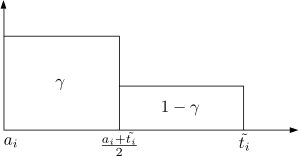
\includegraphics{fig/gendreau2006_distribution.png}
    \caption{Distribuição do limite inferior da janela de tempo de coleta dos
             pedidos \cite{gendreau_neighborhood_2006}}
    \label{fig:gendreau2006_distribution}
\end{figure}

Em que, $\mu$ simboliza a probabilidade do limite inferior da janela de
tempo de coleta estar contido no intervalo 
$[\arrivalTime_\request; \frac{\arrivalTime_\request + \Tilde{t}_\request}{2}]$
, e é definodo por:

\begin{equation}
  \mu = \uniformDistribution{0,6}{1,0}
\end{equation}

Já o limite superior da janela de tempo de coleta é definido por:

\begin{equation}
    \latestTimeWindow_\originIndex = 
      \earliestTimeWindow_\originIndex 
      + \tau(\planingHorizon - \arrivalTime_\request),
\end{equation}

em que, $\tau(\planingHorizon - \arrivalTime_\request)$ representa uma fração
do tempo entre o insntate de chegada do pedido e o fim do horizonte de
planejamento. $\tau$ é portanto definido por:

\begin{equation}
  \tau = \uniformDistribution{\tau^{\min}}{\tau^{\max}},
\end{equation}

sendo $\tau^{\min}$ e $\tau^{\max}$ são parâmetros determinados pelo usuário,
cujos valores podem variar com o tempo e localização.

Uma janela de tempo é gerada da mesma forma para o local de entrega. 
Neste caso a distribuição de probabilidade para a geração do limite inferior 
da janela de tempo de entrega, como mostrado na 
Figura~\ref{fig:gendreau2006_distribution}, é definido sobre o intervalo
$[\earliestTimeWindow_\originIndex 
+ \arcTravelTime{\originIndex}{\destinationIndex}^{\min}, 
\Tilde{t} + \arcTravelTime{\originIndex}{\destinationIndex}^{\min}]$.
Já o limite superior da janela de tempo de entrega é também definido como uma
fração do intervalo de tempo entre o limite inferior da janela de tempo de
entrega e o instante final do horizonte de planejamento.

O tempo de serviço é igual a 5 minutos em cada local de serviço e um pedido é 
aceito somente quando existe no mínimo 30 minutos entre o instante de chegada 
do pedido e o último instante de coleta 
($\latestTimeWindow_\request - \requestArrivalTime \geq 30$). 
Os valores para os parâmetros $\tau$ usados para a geração das janelas de tempo
foram tomados a partir do sorteio de distribuições uniformes 
$\uniformDistribution{0,1}{0,8}$ e $\uniformDistribution{0,3}{1,0}$.

A Tabela~\ref{tab:gendreau2006_instances_characteristics} apresenta algumas
características das instâncias apresentadas por
\textcite{gendreau_neighborhood_2006}

\begin{table}[h]
\footnotesize
    \caption{Características das instâncias DPDPTW de 
             \textcite{gendreau_neighborhood_2006}}
    \label{tab:gendreau2006_instances_characteristics}
    \centering
    \begin{tabular}{lrr|lrr}
        \toprule
         ID & $\planingHorizon$ & $\numberOfRequests$ & 
         ID & $\planingHorizon$ & $\numberOfRequests$ \\
         \midrule
         req\_rapide\_1\_240\_24 & 240 &  84 & 
         req\_rapide\_3\_450\_24 & 450 & 206 \\ 
         req\_rapide\_1\_240\_33 & 240 & 144 & 
         req\_rapide\_4\_450\_24 & 450 & 217 \\
         req\_rapide\_1\_450\_24 & 240 & 169 & 
         req\_rapide\_4\_240\_24 & 240 &  90 \\ 
         req\_rapide\_2\_450\_24 & 450 & 176 &
         req\_rapide\_5\_240\_24 & 240 &  85 \\
         req\_rapide\_2\_240\_24 & 240 &  94 &
         req\_rapide\_5\_240\_33 & 240 & 153 \\
         req\_rapide\_2\_240\_33 & 240 & 112 &
         req\_rapide\_5\_450\_24 & 450 & 202 \\
         req\_rapide\_3\_240\_24 & 240 &  93 &
         req\_rapide\_5\_450\_24 & 450 & 202 \\
         req\_rapide\_3\_240\_33 & 240 & 111 &
                                 &     &     \\
         \bottomrule
  \end{tabular}
\end{table}

\iffalse




\section{Conjunto de instâncias DPDPTW propostas por 
         Mitrovic-Minic e Laporte (2004) e Mitrovic-
         Minic, Krishnamurti e Laporte (2004)}

Composto por dois subconjuntos de instâncias, cada um contendo 30 instâncias de 
100, 30 de 500 e 30 de 1000 pedidos.
Estes conjuntos diferem apenas em relação à distribuição e largura das 
janelas de tempo, que dependem do tempo máximo permitido para servir o pedido, 
assumindo que o pedido é coletado no primeiro instante possível, e são dadas 
por:

\begin{equation}
    \Gamma = \latestTimeWindow_{\destinationIndex}
              - \earliestTimeWindow_\originIndex.
    \label{eq: mitrovic_maximal_time_allowed}
\end{equation}

Os pedidos são gerados baseados em dados reais coletados em duas companhias de 
correio de médio e grande porte que operam em Vancouver, Canadá.
No primeiro conjunto a distribuição de pedidos é representada por: 
20\% pedidos com $\Gamma$ = 1 h, 30\% pedidos com $\Gamma$ = 2 h e 
50\% pedidos com $\Gamma$ = 4 h.
No segundo conjunto a distribuição é representada por: 10\% dos pedidos com 
$\Gamma$ = 1 h, 20\% dos pedidos com $\Gamma$ = 2 h, 30\% dos pedidos com 
$\Gamma$ = 4 h, 30\% dos pedidos com $\Gamma$ = 6 h 
e 10\% dos pedidos com $\Gamma$ = 8 h.

O horizonte de planejamento é de 10 h, a área de serviço é de $60 \times 60$ 
km$^2$, e a velocidade do veículo é de 60 km/h. 
Os instantes de chegada dos pedidos ocorrem dentro do horizonte de planejamento
de acordo com uma distribuição uniforme contínua e nenhum pedido é conhecido 
a priori,

\begin{equation}
  \arrivalTime_\request = \uniformDistribution{0}{\planingHorizon}.
\end{equation}


Um pedido $\request$ é criado através da seguinte sequência de procedimentos: 
(i) gerar o instante de chegada, 
(ii) gerar aleatoriamente as posições de coleta e entrega e 
(iii) gerar um valor para $\Gamma$.
(iv) calcular os limites das janelas de tempo como:

\begin{equation}
  \earliestTimeWindow_\originIndex = \arrivalTime_\request,
\end{equation}

\begin{equation}
  \latestTimeWindow_{\destinationIndex} = \earliestTimeWindow_\originIndex +
  \Gamma,
\end{equation}

\begin{equation}
  \latestTimeWindow_\originIndex = \latestTimeWindow_{\destinationIndex}
  - \arcTravelTime{i}{i+n},
\end{equation}

\begin{equation}
  \earliestTimeWindow_{\destinationIndex} = \earliestTimeWindow_\originIndex
  + \arcTravelTime{i}{i+n}.
\end{equation}


Rejeições de pedidos e violações de janelas de tempo não são permitidas. 
Isso é feito possível pelo fato que a quantidade de veículos 
($\vehiclesSetSize$) é considerada ilimitada. 
A frota inicial é considerada 20, 60 e 80 para as instâncias com 100, 500 e 
1000 pedidos, respectivamente. 
O ponto de início é posicionado em (20, 30) km.


\fi



    % Primeiro capitulo de Resultados
    \chapter{Medidas}\label{ch:medidas}
% TODO Introduzir o que seriam medidas e a importância delas para as pesquisas 
% com relação a roteamento dinâmico de veículos

% TODO adicionar outros exemplos de medidas, explicando para que servem

% TODO explicar o porque dinamismo e urgência foram escolhidas

Proposta primeiramente por \citeonline{lund_vehicle_1996}, o grau de dinamismo
de uma instância de qualquer VRP dinâmico representa a razão entre a quantidade
de pedidos dinâmicos, que se fazem conhecidos em um instante
$\arrivalTime_\request > 0$, e a quantidade total de pedidos da instância.

\begin{equation}
  \degreeOfDynamism = \frac{\numberOfRequests_{d}}{\numberOfRequests}.
  \label{eq:degreeOfDynamism}
\end{equation}

Em que:
\begin{itemize}
  \item $\degreeOfDynamism$: grau de dinamismo
  \item $\numberOfRequests_{d}$: número de pedidos dinâmicos
\end{itemize}

Essa classificação proporcionou uma base para o estudo das relações entre o 
grau de dinamismo, os tipos de métodos usados para a solução dos 
problemas e as características das soluções obtidas.
\citeonline{wong_dynamic_2014}, por exemplo, mostram que existe uma relação não
linear entre o grau de dinamismo e o custo de transporte de uma instância de um
problema DRT.
Suas análises numéricas elucidam a existência de um pico de ineficiência para
vários algorítimos heurísticos quando $\degreeOfDynamism \approx 0{,}7$.
Através dessa descoberta \citeonline{wong_dynamic_2014} descrevem uma série de
políticas para que operadores de sistemas de transporte responsivos a demanda
(DRT) possam seguir para permanecer longe do que eles classificam como "zona de
dilema".

Similarmente, \citeonline{larsen_partially_2002} usam essa mesma medida de 
grau de dinamismo para estudar a relação entre o custo de rota para o 
problema parcialmente dinâmico do reparador itinerante 
(PDTRP - \textit{Partially Dynamic Traveling Repairman Problem}).
Os resultados empíricos ilustram uma relação linear entre o nível de
dinamismo de uma instância e o custo da rota de um sistema relativamente ativo.

Posteriormente, baseando-se no fato de que o instante de chegada dos pedidos
dinâmicos também deve afetar o grau de dinamismo,
\citeonline{larsen_dynamic_2000} define o grau efetivo de dinamismo por:

\begin{equation}
  \eDegreeOfDynamism = 
  \frac{1}{\numberOfRequests}
  \sum_{\request \in \requests}
  {
    \frac{\arrivalTime_\request}{\planingHorizon}
  }.
  \label{eq:eDegreeOfDynamism}
\end{equation}

Em que:
\begin{itemize}
  \item $\eDegreeOfDynamism$: grau efetivo de dinamismo
\end{itemize}

O grau efetivo de dinamismo representa a média da razão entre os instantes que
os pedidos são conhecidos quando comparados com o último instante possível para
a chegada deles, $\planingHorizon$, no caso.
Os instantes de chegada dos pedidos estáticos são considerados igual a zero.
É importante destacar que apesar de representarem formas de cálculo diferentes
o grau de dinamismo e o grau de dinamismo efetivo compartilham entre si o mesmo
intervalo de possíveis valores, contido entre $0$ e $1$, sendo que
$\degreeOfDynamism = \eDegreeOfDynamism = 0$ classifica uma instância
totalmente estática e $\degreeOfDynamism = \eDegreeOfDynamism = 1$ representa
uma totalmente dinâmica.

Em um outro estudo, \citeonline{larsen_classification_2007} usam o grau efetivo
de dinamismo para classificar os problemas DVRP em três classes distintas:
fracamente, moderadamente e fortemente dinâmicos, cujos intervalos de valores 
$\eDegreeOfDynamism$ correspondem, respectivamente, a $\eDegreeOfDynamism \leq
0{,}3$, $0{,}3  < \eDegreeOfDynamism < 0{,}8$ e $0{,}8 \leq
\eDegreeOfDynamism$.
A intenção dessa segregação de problemas é facilitar a escolha de um algoritmo
para a sua solução.

\citeonline{larsen_dynamic_2000} também estende o grau de dinamismo efetivo
para problemas com janelas de tempo.
A ideia é contabilizar também o nível de urgência de cada um dos pedidos, 
sendo que o nível de urgência é visto como o tempo de reação disponível
para que o sistema, após receber a informação do pedido no instante
$\arrivalTime_\request$, possa passar pelo nó de coleta $\originNode$
antes do limite superior da janela de tempo de coleta
$\latestTimeWindow_{\originIndex}$.
\citeonline{larsen_dynamic_2000} define que: 

\begin{equation}
  \reactionTime_\request = \latestTimeWindow_{\originIndex}
                           - \arrivalTime_\request.
\end{equation}

Em que:
\begin{itemize}
  \item $\reactionTime_\request$: tempo de reação do pedido $\request$
\end{itemize}

Com isso, o grau efetivo de dinamismo, quando contabilizado o tempo de reação,
é definido por \citeonline{larsen_dynamic_2000}:

% TODO tentar alinhar os sinais de igualdade das duas equações a seguir

\begin{equation}
  \eDegreeOfDynamismTW := 
  \frac{1}{\numberOfRequests}
  \sum_{\request \in \requests}
  {
    \left(
    \frac{\planingHorizon - (\latestTimeWindow_\originIndex
                             - \arrivalTime_\request)}
         {\planingHorizon}
    \right),
  }
\end{equation}

\begin{equation}
  \eDegreeOfDynamismTW := 
  \frac{1}{\numberOfRequests}
  \sum_{\request \in \requests}
  {
    \left(
      1 - \frac{\reactionTime_\request}{\planingHorizon}
    \right).
  }
\end{equation}

Em que:
\begin{itemize}
  \item $\eDegreeOfDynamismTW$: grau efetivo de dinamismo com janelas de tempo
\end{itemize}

É importante destacar que, assim como as medidas apresentadas anteriormente, o
grau efetivo de dinamismo com janelas de tempo também apresenta valores somente
dentro do intervalo $[0, 1]$.

\citeonline{pillac_review_2013} relata que todas as três medidas expostas nesse
capítulo se provaram úteis para capturar os aspectos do dinamismo relacionados
com o tempo.
Entretanto essas medidas não levam em consideração outras fontes de dinamismo,
como a distribuição espacial dos pedidos e o tempo de viagem entre pedidos.
Essas fontes de dinamismo se mostram bastante importantes quando o objetivo é
minimizar o tempo de resposta do sistema.

Além disso, apesar de não considerada na definição das medidas de dinamismo, a
frequência com que os pedidos chegam ao sistema tem um grande impacto no tempo
disponível para otimização \cite{pillac_review_2013}.
Similarmente, \citeonline{kilby_dynamic_1998} fazem a observação de que a
frequência dos pedidos influencia na quantidade de vezes que o algoritmo
precisa ser refeito.
Eles destacam que instâncias em que os pedidos estão agrupados em
pequenos intervalos de tempo geram menos necessidade de reoptimização do que
casos onde os pedidos estão separados um dos outros de maneira uniforme.

No final do seu artigo, \citeonline{larsen_classification_2007} recomendam, 
para futuras pesquisas, a extensão do grau de dinamismo para que ele também 
leve em conta outras características do problema, como o tamanho dos tempos de 
serviço e o carregamento dos pedidos.
Eles também mencionam que é desafiador encontrar uma medida única para 
apreender múltiplas características de uma instância.

Com o intuito de produzir medidas que melhor representam as características
relacionadas ao dinamismo de um DPDPTW, \citeonline{van_lon_measures_2016} 
propõem uma nova definição para a medida de dinamismo, como também uma nova
medida denominada urgência.
Apesar do foco ser em problemas DPDPTW, \citeonline{van_lon_measures_2016}
afirmam que os conceitos de dinamismo e urgência não são limitados a este tipo
de problema, podendo ser usados em qualquer DVRP.

Como premissa, os autores consideram que estes parâmetros devem ser 
relacionados apenas ao problema, e portanto, o algoritmo usado para solução 
não deve influenciar em seus valores.
Entretanto, é desejado que essas medidas colaborarem para a classificação das 
instâncias e assim permitam a análise da eficácia dos algoritmos quando 
submetidos a diferentes condições de dinamismo e urgência. 
Além disso, \citeonline{van_lon_measures_2016} afirmam que as medidas devem ser 
interdependentes, não podendo haver correlação entre suas definições. 

O restante desse capítulo apresenta a definição, feita por
\citeonline{van_lon_measures_2016}, das duas medidas usadas para a determinação
das características temporais dos pedidos de uma instância de um problema de 
roteamento dinâmico qualquer.
Posteriormente, no Capítulo~\ref{ch:analise} usa-se essas medidas para analisar
e comparar os conjuntos de instância de \textit{benchmark} expostos no 
Capítulo~\ref{ch:instancias}.






\section{Dinamismo}\label{sec:dinamismo}
Define-se, primeiramente, que o grau de dinamismo é dado através da 
continuidade de mudança das informações presentes para um sistema. 
Por esse ponto de vista, todo evento que introduz informações novas para o 
problema, como a chegada de um pedido, a quebra de um veículo ou o cancelamento
de uma viagem, é classificado como uma mudança.
Um cenário muito dinâmico é caracterizado por mudanças contínuas, em oposição a
um cenário pouco dinâmico, onde mudanças ocorrem ocasionalmente.
A Figura~\ref{fig:van_lon_measures_2016_dynamism} demonstra, 
através de exemplos, as diferentes formas de distribuição de mudanças,
associando cada uma à um grau de dinamismo.

% TODO: mudar para arquivo .eps
\begin{figure}[H]
    \begin{center}
        \makebox[\textwidth]
          {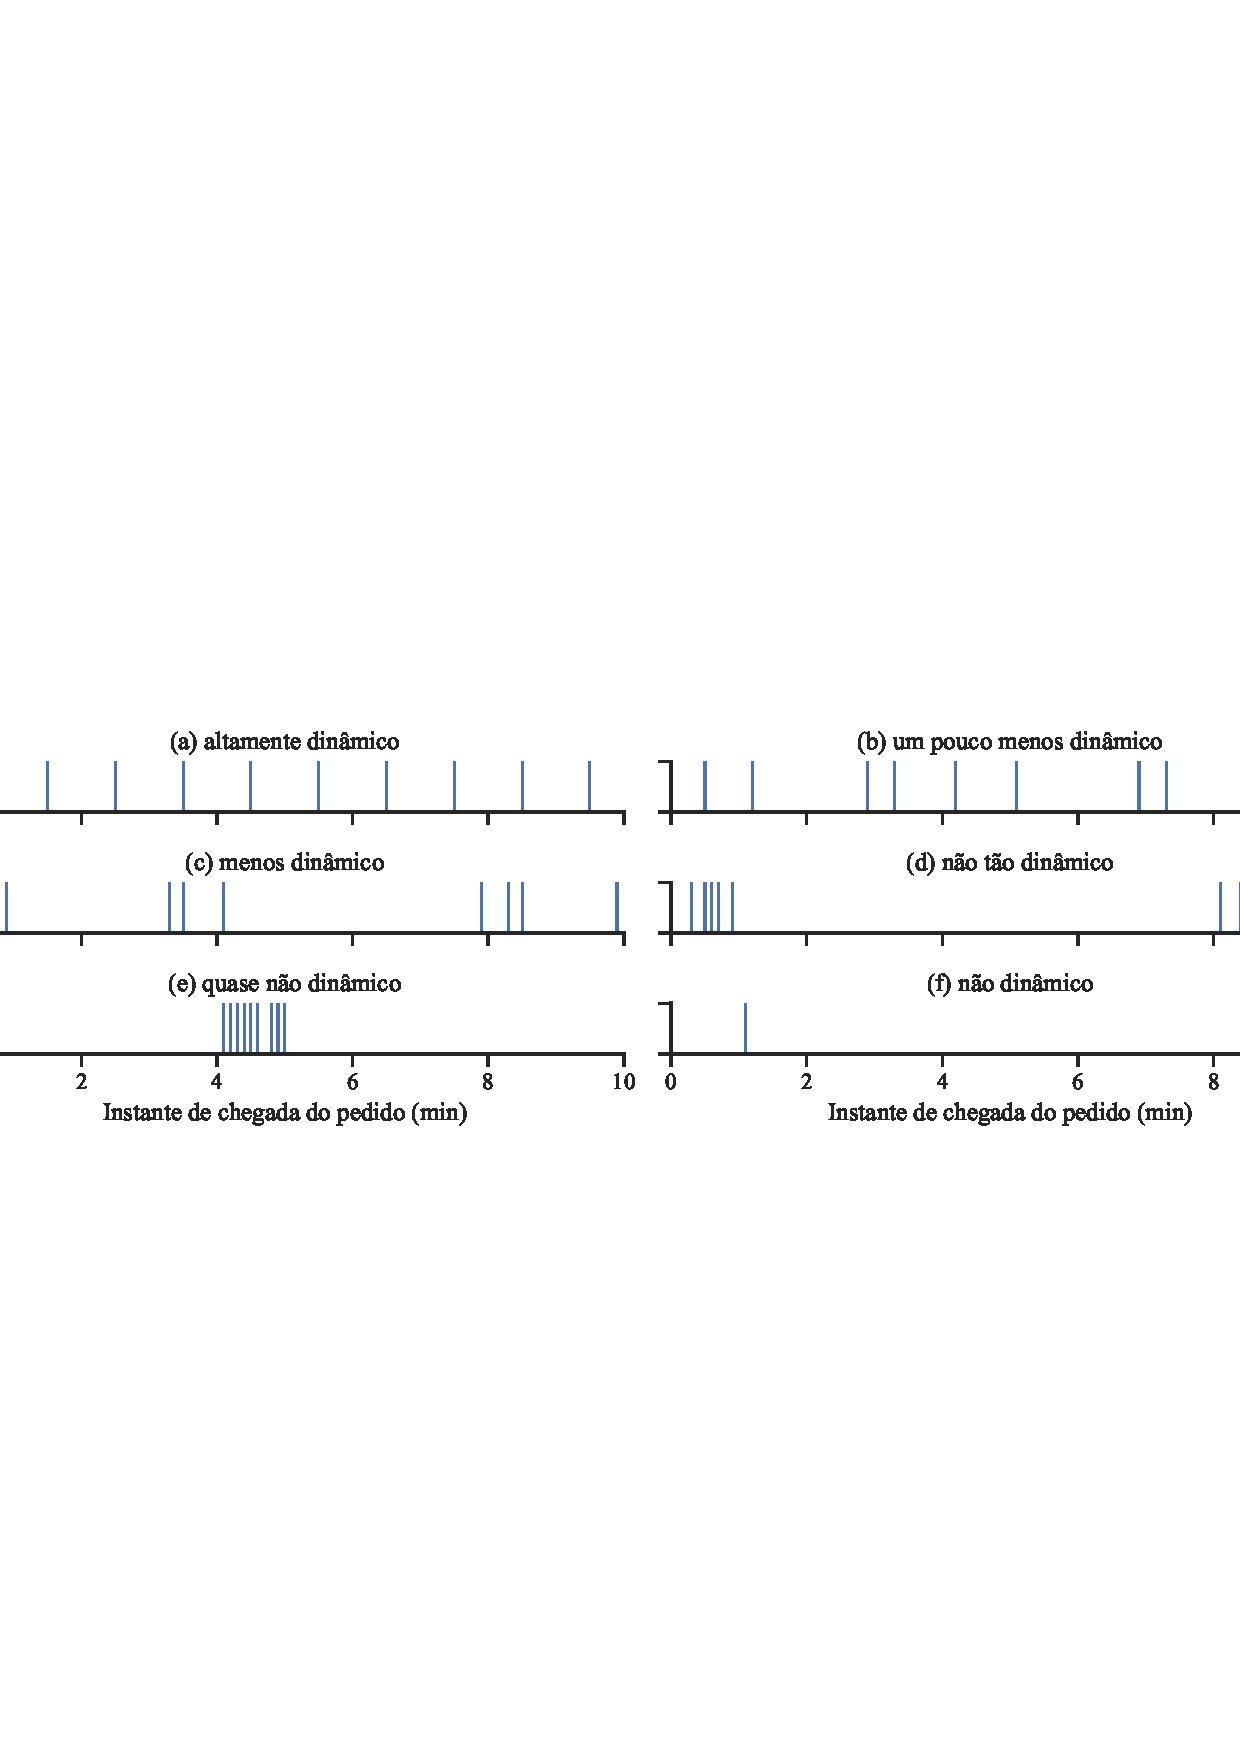
\includegraphics[width=\textwidth]{./fig/dynamism_sample.png}}
        \caption{Exemplos de cenários com diferentes valores de dinamismo 
        \cite{van_lon_measures_2016}}
        \label{fig:van_lon_measures_2016_dynamism}
    \end{center} 
\end{figure}

Todos os gráficos da Figura~\ref{fig:van_lon_measures_2016_dynamism},
identificados pelas letras (a-f), representam um cenário com horizonte de 
planejamento de 10 minutos e com um total de 10 pedidos dinâmicos.
No cenário Figura~\ref{fig:van_lon_measures_2016_dynamism}(a) os eventos 
acontecem em intervalos igualmente espaçados e distribuídos proporcionalmente 
no horizonte de planejamento.
Nos cenários Figura~\ref{fig:van_lon_measures_2016_dynamism}(b, c) pode-se ver
que mudanças ocorrem com menos frequência.
Em Figura~\ref{fig:van_lon_measures_2016_dynamism}(d, e) todos os eventos
ocorrem em uma ou duas bateladas, fazendo-os menos contínuos e portanto menos
dinâmicos.
Em Figura~\ref{fig:van_lon_measures_2016_dynamism}(f) todos os eventos chegam
em um mesmos instante, resultando em um cenário sem dinamismo
\cite{van_lon_measures_2016}.

Para formular a medida de dinamismo \citeonline{van_lon_measures_2016} define
primeiramente uma lista, $\intervalsBetweenArrivals$, de intervalos de chegadas 
entre pedidos:

\begin{equation}
    \intervalsBetweenArrivals = 
    \{\intervalBetweenArrivals_0,\intervalBetweenArrivals_1,\ldots, 
    \intervalBetweenArrivals_{\numberOfRequests-2}\} = 
    \{\arrivalTime_j - \arrivalTime_i 
    \mid j = i + 1 \wedge \forall i, j \in \pickupNodes\},
    \label{eq:van_lon_measures_2016_intervalsBetweenArrivals}
\end{equation}

\begin{equation}
    |\intervalsBetweenArrivals| = \numberOfRequests - 1.
    \label{eq:van_lon_measures_2016_intervalsBetweenArrivalsSize}
\end{equation}

Em que:
\begin{itemize}
  \item $\intervalsBetweenArrivals$: lista de intervalos entre chegada de 
    pedidos.
  \item $\intervalBetweenArrivals_\request$: intervalo de tempo entre a chegada
    do pedido $\request$ e seu sucessor.
\end{itemize}

Portanto, $\intervalsBetweenArrivals$ representa uma lista com todos os valores
de intervalos de tempo em que o estado do sistema não é alterado, ordenados
cronologicamente.
Essa lista possui uma quantidade de valores $|\intervalsBetweenArrivals|$ 
cuja definição é apresentada na
Equação~\ref{eq:van_lon_measures_2016_intervalsBetweenArrivalsSize}

Para motivos de comparação, é definido um intervalo de chegada perfeito,
$\perfectInterval$. Este é dado por:

\begin{equation}
    \perfectInterval = \frac{H}{\numberOfRequests}.
    \label{eq:van_lon_measures_2016_perfectInterval}
  \end{equation}

Em que:
\begin{itemize}
  \item $\perfectInterval$: intervalo de chegada perfeito
\end{itemize}

Com isso obtêm-se o espaço de tempo entre pedidos do cenário com maior
dinamismo possível, dada uma quantia de pedidos $\numberOfRequests$ 
e um horizonte de planejamento $\planingHorizon$.
Voltando ao exemplo da Figura~\ref{fig:van_lon_measures_2016_dynamism},
temos que o cenário (a) seria o cenário em que
$\intervalBetweenArrivals_\request = \perfectInterval, \forall
\intervalBetweenArrivals_\request \in \intervalsBetweenArrivals$.
Ou seja, dos cenários apresentados na 
Figura~\ref{fig:van_lon_measures_2016_dynamism}, o cenário (a) é, além do mais
dinâmico dos cenários da figura, também o cenário mais dinâmico possível pra
esses valores de $\numberOfRequests$ e $\planingHorizon$.

Tendo os conceitos de intervalos entre chegadas de pedido e o intervalo de
chegada perfeito definidos, pode-se definir o desvio,
$\deviationFromPerfectInterval$, entre os intervalos de chegada contidos em
$\intervalsBetweenArrivals$ com o intervalo de chegada perfeito,
$\perfectInterval$:

\begin{equation}
    \deviationFromPerfectInterval_i =
        \begin{cases}
            \perfectInterval - \intervalBetweenArrivals_i,
            & \text{se $i = 0$ 
                    e $\intervalBetweenArrivals_i < \perfectInterval$} \\
            \perfectInterval - \intervalBetweenArrivals_i 
            + \frac{\perfectInterval-\intervalBetweenArrivals_i}
                   {\perfectInterval}
            \cdot \deviationFromPerfectInterval_{i-1},
            & \text{se $i > 0$ 
                    e $\intervalBetweenArrivals_i < \perfectInterval$} \\
            0, & \text{do contrário.}
        \end{cases}
    \label{eq:van_lon_measures_2016_deviationFromPerfectInterval}
\end{equation}

Em que:
\begin{itemize}
  \item $\deviationFromPerfectInterval_i$: desvio entre os intervalo de chegada
    $\intervalBetweenArrivals_i$ e o $\perfectInterval$
\end{itemize}

Sendo que o termo $\frac{\perfectInterval-\intervalBetweenArrivals_i}
{\perfectInterval} \cdot \deviationFromPerfectInterval_{i-1}$ serve para 
penalizar, de forma recursiva, a aglutinação de eventos em pequenos 
períodos de tempo.

% TODO: explicar melhor o que significa cada um dos casos da equação acima,
% assim como o conceito completo expresso por ela.

Consequentemente, o desvio total do cenário pode ser calculado por:

\begin{equation}
    \deviation = 
    \sum_{i=0}^{|\intervalsBetweenArrivals|} \deviationFromPerfectInterval_i.
    \label{eq:van_lon_measures_2016_totalDeviationFromPerfectInterval}
\end{equation}


Entretanto, faz-se necessária a normalização do desvio total do cenário com
relação ao desvio máximo possível.
Para isso, calcula-se o maior valor:

\begin{equation}
    \maxDeviation =
    \sum_{i=0}^{|\intervalsBetweenArrivals|} 
		\overline{\deviationFromPerfectInterval}_i,
    \label{eq:van_lon_measures_2016_bigestTotalDeviationFromPerfectInterval}
\end{equation}

em que:

\begin{equation}
    \overline{\deviationFromPerfectInterval}_i = \perfectInterval + 
        \begin{cases}
            \frac{\perfectInterval - \intervalBetweenArrivals_i}
								 {\perfectInterval} 
						\cdot \deviationFromPerfectInterval_{i-1},
						& \text{se $i>0$ e $\intervalBetweenArrivals_i 
                    < \perfectInterval$}\\
            0, & \text{do contrário.}
        \end{cases}
    \label{eq:van_lon_measures_2016_bigestDeviationFromPerfectInterval}    
\end{equation}

Combinando as 
Equações~\ref{eq:van_lon_measures_2016_bigestTotalDeviationFromPerfectInterval}
e~\ref{eq:van_lon_measures_2016_bigestDeviationFromPerfectInterval}, define-se 
dinamismo como:

\begin{equation}
      \dynamism = 1 - \frac{\deviation}{\maxDeviation} = 1 -
      \frac{\sum_{i=0}^{|\intervalsBetweenArrivals|}
			\deviationFromPerfectInterval_i}{\sum_{i=0}^{|\intervalsBetweenArrivals|}
      \overline{\deviationFromPerfectInterval}_i}.
      \label{eq:van_lon_measures_2016_dynamism}
\end{equation}

% TODO: Escrever interpretação das 4 equações anteriores






\section{Urgência}\label{sec:urgencia}

No contexto dos DVRPs, a urgência representa o tempo de reação disponível ao 
sistema de trasporte para que ele consiga atender a um pedido.
Essa medida pode ser expressa através de unidades de tempo e definida pela 
diferença entre o instante de chegada de um pedido ($\arrivalTime_\request$) 
e o limite superior da janela de tempo de coleta 
($\latestTimeWindow_\originIndex$).
A Figura~\ref{fig:van_lon_measures_2016_urgency} exemplifica dois casos.

%TODO: converter imagem de png para eps
\begin{figure}[H]
    \begin{center}
        \makebox[\textwidth]{
          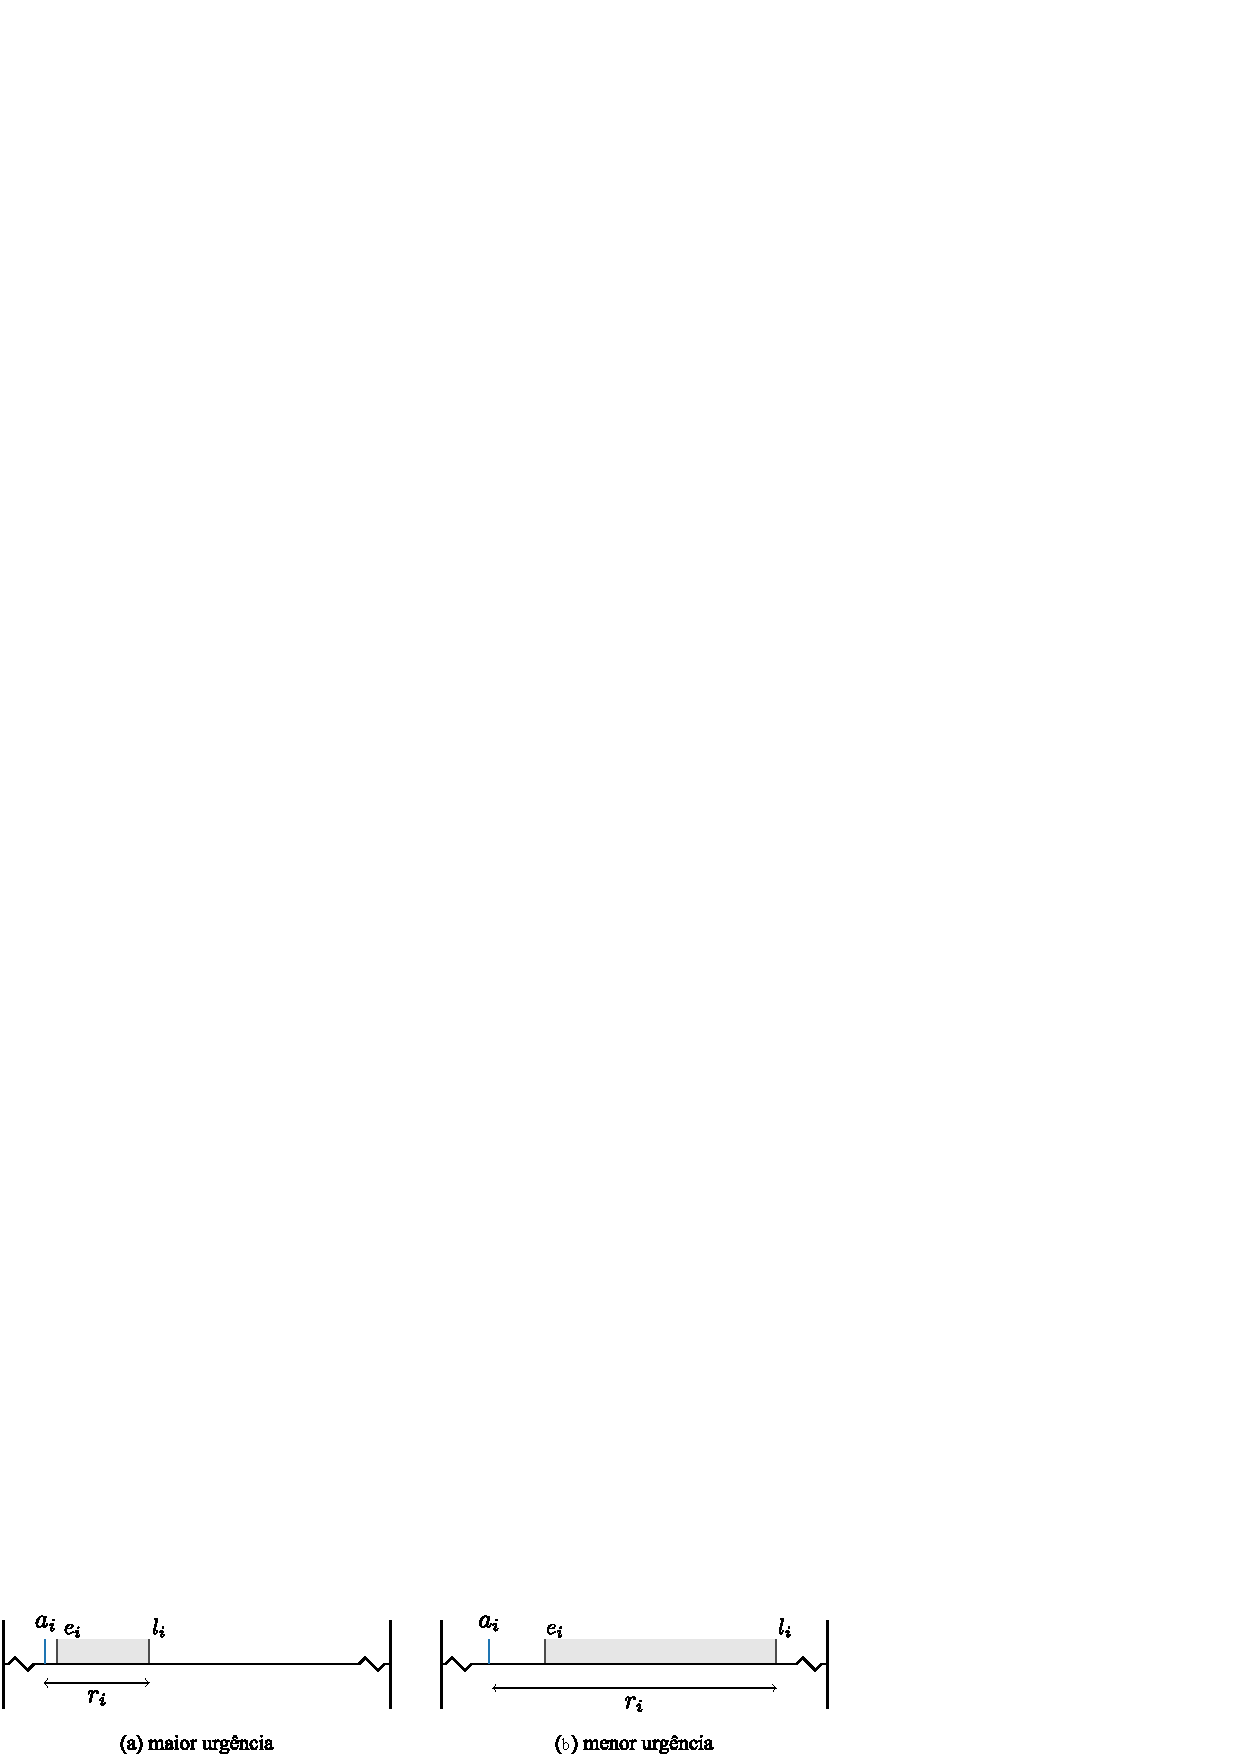
\includegraphics[width=\textwidth]{fig/urgency_sample.png}}
        \caption{Exemplos de pedidos com diferentes valores de urgência 
                 \cite{van_lon_measures_2016}}
        \label{fig:van_lon_measures_2016_urgency}
    \end{center} 
\end{figure}

No cenário Figura~\ref{fig:van_lon_measures_2016_urgency}(a) temos o exemplo de
um pedido com grande urgência, ou seja, menor tempo de reação.
Já no caso Figura~\ref{fig:van_lon_measures_2016_urgency}(b) o tempo de reação
é menor, portanto o pedido é menos urgente.

Baseando-se na Figura~\ref{fig:van_lon_measures_2016_urgency}, 
\citeonline{van_lon_measures_2016} define urgência por:

\begin{equation}
    \urgency_\request = \latestTimeWindow_\request - \arrivalTime_\request.
    \label{eq:van_lon_measures_2016_urgency}
\end{equation}

Em que:
\begin{itemize}
  \item $\urgency_\request$: urgência do pedido $\request$
\end{itemize}

Para obter uma indicação da urgência de um cenário completo, pode-se computar a
média e o desvio padrão das urgências. 
Esta definição é similar ao grau de dinamismo efetivo com janelas de tempo 
proposto por \citeonline{larsen_dynamic_2000} e definido nas
Equações~\ref{eq:degreeOfDynamism}~e~\ref{eq:eDegreeOfDynamism}.
Entretanto, exite uma diferença entre estas duas definições.
\citeonline{larsen_dynamic_2000} normaliza os valores do grau de dinamismo
efetivo com janelas de tempo usando o horizonte de planejamento.  
Já \citeonline{van_lon_measures_2016} acredita que a extensão do cenário e
a urgência devem ser independentes.




    % Segundo capitulo de Resultados
    \chapter{Análise dos Conjuntos de \textit{Benchmark}}\label{ch:analise}

Neste capítulo as métricas apresentadas no Capítulo~\ref{ch:medidas} são 
utilizadas para analisar as instâncias de \textit{benchmark} descritas no
Capítulo~\ref{ch:instancias}. 
Esta análise tem como objetivo avaliar a dispersão dos valores de dinamismo e 
urgência das instâncias de cada conjunto de \textit{benchmark} e com isso 
permitir que futuras pesquisas possam se basear nos
dados expostos nesse capítulo para escolher conjuntos de \textit{benchmark} que
representem cenários de interesse prático para teste.






\section{Distribuição do grau de dinamismo e da urgência}

Cada um dos gráficos apresentados na 
Figura~\ref{fig:scatterplot_instance_planing_horizon} representa um conjunto 
de instâncias de \textit{benchmark} diferente. 
Cada ponto no gráfico corresponde aos valores de urgência média normalizada 
(eixo vertical) e dinamismo (eixo horizontal) de uma das instâncias desse 
conjunto.
A normalização da urgência média é feita de maneira que o valor zero represente
uma urgência média igual a zero e o valor um represente a maior urgência média
encontrada dentro do conjunto de instâncias de \textit{benchmark} em questão.
A figura mostra o acúmulo dos pontos, o que demonstra a falta
de diversidade entre instâncias de um mesmo conjunto de \textit{benchmark},
para os critérios considerados.

% TODO Rodrigo: porque o que está relatado no parágrafo anterior é ruim?

A Figura~\ref{fig:dynamism_boxplot_planing_horizon} mostra os mesmos valores de
dinamismo exibidos na Figura~\ref{fig:scatterplot_instance_planing_horizon}, 
entretanto em forma de diagrama de caixas, em que 50\% dos valores de dinamismo
de cada conjunto de \textit{benchmark} estão contidos nas caixas.
A mediana dos valores é demarcada por um risco vertical dentro desta caixa e os
limites inferiores ($LI$) e superiores ($LS$) são demarcados pelos segmentos 
de reta vertical externos às caixas, cujos valores podem ser calculados 
por:
%
\begin{equation}
  LI = Q_1 - 1{,}5 \cdot AIQ,
\end{equation}
%
\begin{equation}
  LS = Q_3 + 1{,}5 \cdot AIQ,
\end{equation}
%
\begin{equation}
  AIQ = Q_3 - Q_1,
\end{equation}

\noindent em que $Q_1$ é o primeiro quartil, correspondendo a 25\% das menores 
medidas, $Q_3$ é o terceiro quartil, correspondendo a 75\% das menores medidas
e $AIQ$ é a amplitude interquartil. Ainda no gráfico de caixas, podem ser 
encontrados pequenos losangos, indicando valores não contidos no intervalo 
$[LI; LS]$.

Pode-se observar que quatro dos seis conjuntos estudados possuem medianas 
menores que 0,1 e uma alta concentração de instâncias com dinamismo menor que 
0,2, indicando uma falta de diversificação das instâncias desses quatro 
conjuntos. 
Vale destacar que quanto maior o dinamismo, maior a quantidade de vezes que
necessita-se usar o algoritmo de otimização.
Portanto, conjuntos de \textit{benchmark} com baixo valor de dinamismo podem
beneficiar algoritmos que retornem bons resultados a custo de um longo tempo de
computação.

Outro fator interessante a se destacar é a escassez de instâncias com dinamismo
entre 0,45 e 0,6. 
\citeonline{van_lon_measures_2016} afirmam que este intervalo de valores de 
dinamismo ocorre em cenários gerados por distribuições Poisson homogêneas.
Tendo em vista que as chegadas de pedidos de viagem em sistemas de 
\textit{dial-a-ride} acontecem de forma a se assemelhar com uma distribuição de
Poisson homogênea \cite{schilde_metaheuristics_2011}, a falta de instâncias 
com esses valores de dinamismo prejudica a análise de cenários realísticos.

% TODO mudar imagem para .eps
\begin{figure}[H]
    \centering
    \makebox[\textwidth]
    {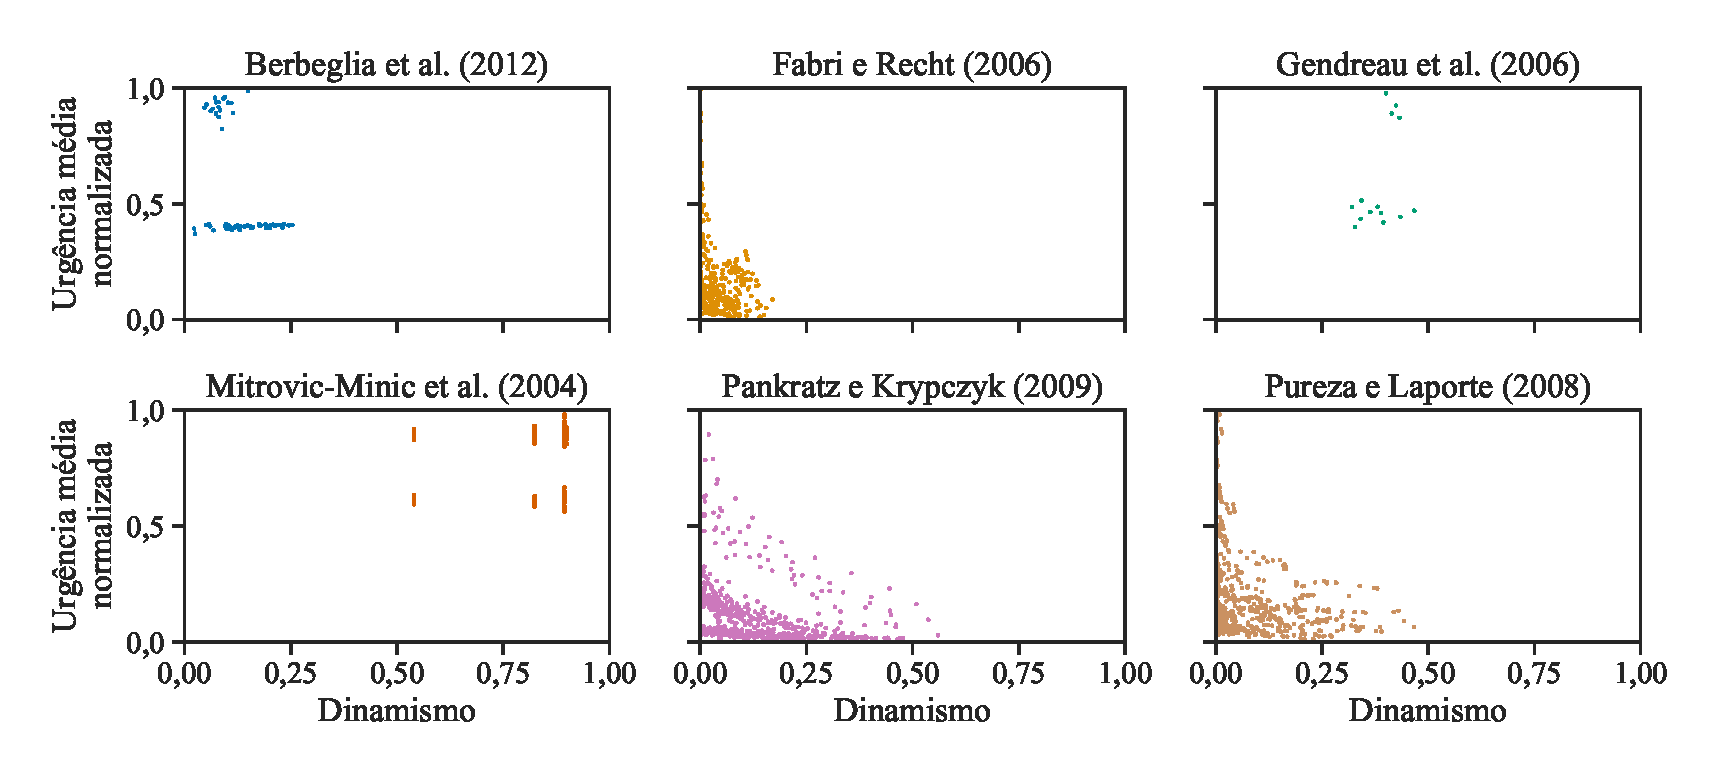
\includegraphics[width=\textwidth]
    {fig/analyses/scatterplot_dynamism_x_urgency_mean_norm_max_planing_horizon.png}}
    \caption{Gráfico de dispersão da urgência média e do dinamismo de cada 
    conjunto de \textit{benchmark}}
    \label{fig:scatterplot_instance_planing_horizon}
\end{figure}

% TODO mudar imagem para .eps
\begin{figure}[H]
    \centering
    \makebox[\textwidth]
    {\includegraphics[width=\textwidth]
    {fig/analyses/boxplot_dynamism_by_benchmark_planing_horizon.png}}
    \caption{Diagrama de caixa dos valores de dinamismo por \textit{benchmark}}
    \label{fig:dynamism_boxplot_planing_horizon}
\end{figure}





\section{Correlação entre os limites inferiores das janelas de tempo de coleta 
e os instantes de chegada dos pedidos}

Pela definição de dinamismo apresentada na Seção~\ref{sec:dinamismo}, os 
intervalos entre os instantes de chegada dos pedidos são os principais fatores
determinadores do valor de dinamismo de uma instância.
Portanto, para que um conjunto de \textit{benchmark} possua instâncias cujos 
valores de dinamismo sejam distintos entre si, se faz necessário que a 
distribuição dos instantes de chegada seja diferente entre instâncias 
\cite{van_lon_measures_2016}.

Entretanto, no Capítulo~\ref{ch:instancias}, percebe-se que grande parte dos 
conjuntos de \textit{benchmark} apresentados um único método de 
dinamização, não possibilitando a diversificação do tamanho dos intervalos de 
tempo entre instâncias.
A única exceção é o método de \citeonline{pankratz_benchmark_2009} que varia o 
valor $\maneuverTime$ garantido a geração de instâncias cujos instantes de 
chegadas diferem entre si.
Porém, mesmo variando esse valor, não foi alcançada uma dispersão grande 
dos valores de dinamismo entre cenários 
(Figuras~\ref{fig:scatterplot_instance_planing_horizon}~e
\ref{fig:dynamism_boxplot_planing_horizon}).

Dentre os métodos de dinamização apresentados no Capítulo~\ref{ch:instancias} é 
comum a utilização dos limites da janela de tempo de coleta para o cálculo dos 
instantes de chegada dos pedidos.
O objetivo do uso deste parâmetro na hora de computar o instante de chegada do 
pedido é garantir que os pedidos possam ser atendidos em tempo hábil.
Entretanto, isso faz com que a distribuição das janelas de tempo das instâncias
estáticas influenciem altamente na distribuição dos instantes de chegadas nos 
pedidos.
Portanto, se a distribuição dos limites das janelas de tempo possuir acúmulo 
de valores, pode-se esperar que os instantes de chegada dos pedidos também  
possua o mesmo acúmulo.

% TODO Rodrigo: pouco visual. Exemplo?

As Figuras~\ref{fig:hist_pickup_lower_tw}~e~\ref{fig:hist_pickup_upper_tw} 
apresentam a distribuição dos limites inferiores e superiores das janelas de 
tempo de coleta de cada um dos conjuntos de \textit{benchmark} normalizados 
pelos horizontes de planejamento de suas respectivas instâncias.
Nota-se que os limites inferiores tendem, em sua maioria, a acumular no início 
do horizonte de planejamento.
Já os limites superiores possuem uma distribuição menos aglutinada, 
porém apresentando ainda pontos de concentração.

% TODO mudar imagem para .eps
\begin{figure}[h]
    \centering
    \makebox[\textwidth]
    {\includegraphics[width=\textwidth]
    {fig/analyses/hist_real_pltw_norm_h_by_benchmark_planing_horizon.png}}
    \caption{Histograma dos limites inferiores das janelas de tempo 
             de coleta por conjunto de \textit{benchmark}}
    \label{fig:hist_pickup_lower_tw}
\end{figure}

% TODO mudar imagem para .eps
\begin{figure}[h]
    \centering
    \makebox[\textwidth]
    {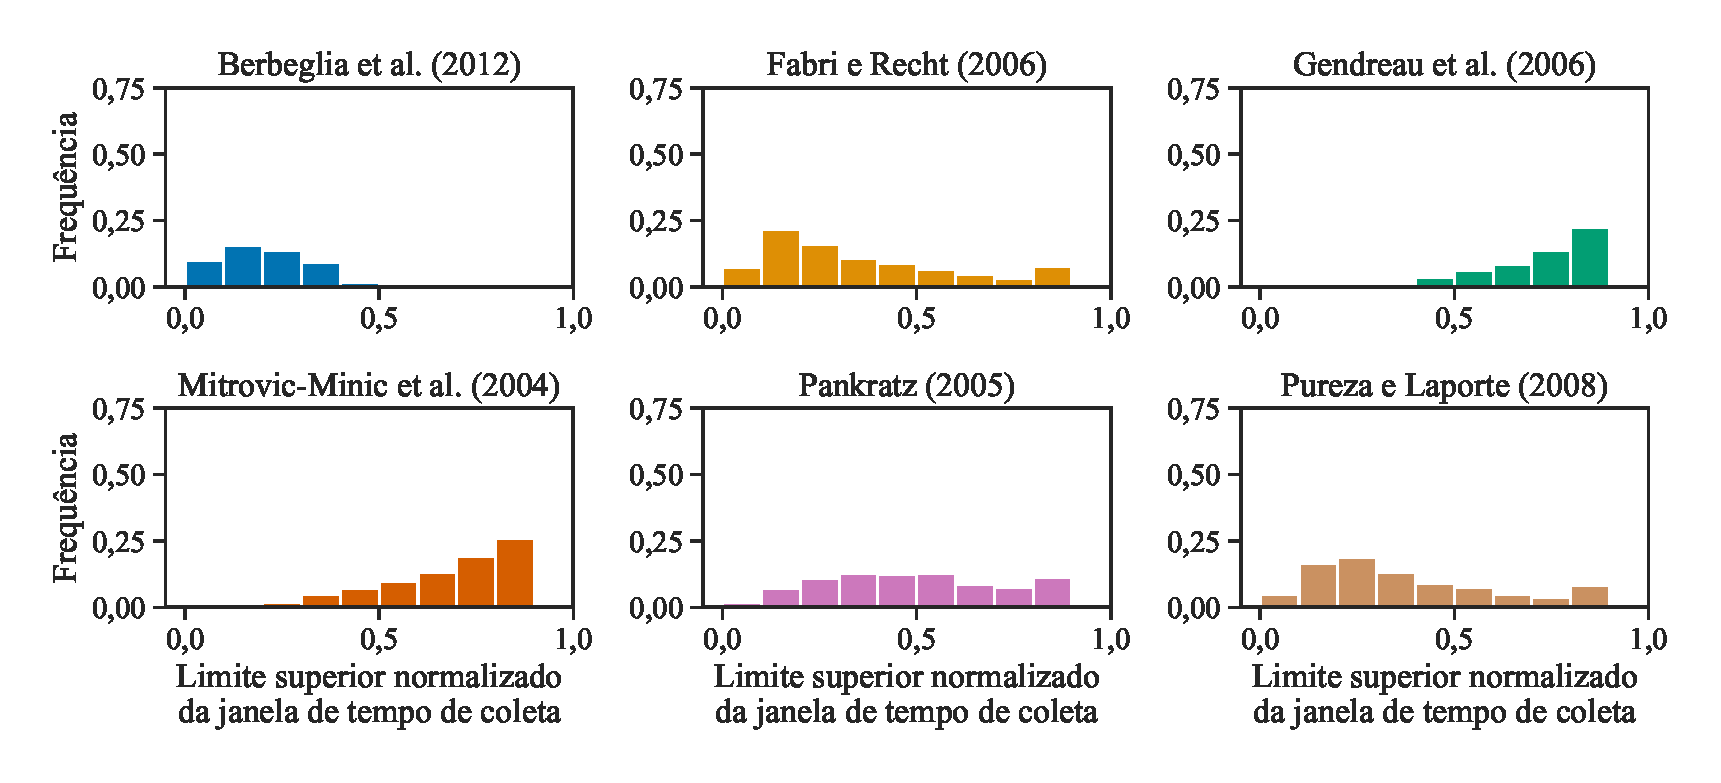
\includegraphics[width=\textwidth]
    {fig/analyses/hist_putw_norm_h_by_benchmark_planing_horizon.png}}
    \caption{Histograma dos limites superiores das janelas de tempo de 
             coleta por conjunto de \textit{benchmark}}
    \label{fig:hist_pickup_upper_tw}
\end{figure}

% TODO Rodrigo: o que tem a ver com as características das instâncias?
% com técnica de dinamização

Como discutido anteriormente, esse acúmulo dos limites da janela de coleta pode
ser propagado para a distribuição dos instantes de chegadas.
Essa propagação pode ser visualizada na Figura~\ref{fig:hist_arrival_time}, que
apresenta as distribuições dos instantes de chegada dos pedidos.
Observa-se que alguns dos acúmulos apresentados nas 
Figuras~\ref{fig:hist_pickup_lower_tw}~e~\ref{fig:hist_pickup_upper_tw} podem 
ser também observados na Figura~\ref{fig:hist_arrival_time}.

% TODO Rodrigo: O que isso quer dizer? Como é feita a propagação?

\begin{figure}[h]
    \centering
    \makebox[\textwidth]
    {\includegraphics[width=\textwidth]
    {fig/analyses/hist_arrival_time_norm_h_by_benchmark_planing_horizon.png}}
    \caption{Histograma dos instantes de chegada para cada conjunto 
             de \textit{benchmark}}
    \label{fig:hist_arrival_time}
\end{figure}

A Tabela~\ref{tab:correlation_real_pltw_norm_h_and_arrival_time_norm_h} 
apresenta, os valores das correlações entre os instantes de chegada dos 
pedidos e os limites inferiores das janelas de tempo de coleta dos pedidos.
Percebe-se uma correlação alta para as instâncias de 
\citeonline{berbeglia_hybrid_tabu_2012}, 
\citeonline{mitrovic-minic_waiting_2004}, 
\citeonline{pankratz_dynamic_2005} e 
\citeonline{pureza_laporte_waiting_2008}.
Já os conjuntos propostos por \citeonline{fabri_dynamic_2006}  e 
\citeonline{gendreau_neighborhood_2006} possuem uma correlação baixa entre estes 
dois parâmetros, que pode ser explicada pelo uso de variáveis aleatórias de 
distribuição uniforme no processo de dinamização ou criação das instâncias.


\begin{table}[H]
    \footnotesize
    \centering
    \caption{Valores de correlação entre os instantes de chegadas normalizados
             e os limites inferiores normalizados das janelas de tempo de
             coleta}
    \label{tab:correlation_real_pltw_norm_h_and_arrival_time_norm_h}
    \begin{tabular}{lr}
        \toprule
        Conjunto de \textit{benchmark}                  & $r$ \\ 
        \midrule
        \citeonline{berbeglia_hybrid_tabu_2012}         & 0,95 \\
        \citeonline{fabri_dynamic_2006}                 & 0,78 \\
        \citeonline{gendreau_neighborhood_2006}         & 0,73 \\
        \citeonline{mitrovic-minic_waiting_2004}        & 1,00 \\
        \citeonline{pankratz_benchmark_2009}            & 0,81 \\
        \citeonline{pureza_laporte_waiting_2008}        & 0,89 \\ 
        \bottomrule
    \end{tabular}
\end{table}


Destaca-se que estes valores de correlação são relativos a uma relação linear
entre as variáveis em questão. Ou seja, ainda podem existir outras relações não
lineares entre o instante de chegada do pedido e o limite inferior da janela
de tempo de coleta.

As Figuras~\ref{fig:scatterplot_pickup_lower_tw_x_arrival_time}~e
\ref{fig:scatterplot_pickup_upper_tw_x_arrival_time} apresentam, 
de forma visual, as correlações entre os instantes de chegada dos 
pedidos e os limites das janelas de tempo de coleta dos pedidos.
Percebe-se uma correlação alta para as instâncias de 
\citeonline{berbeglia_hybrid_tabu_2012}, 
\citeonline{mitrovic-minic_double-horizon_2004}, 
\citeonline{pankratz_benchmark_2009} e 
\citeonline{pureza_laporte_waiting_2008}.
Já os conjuntos propostos por \citeonline{gendreau_neighborhood_2006} e
\citeonline{fabri_dynamic_2006} possuem uma correlação baixa entre estes 
dois valores, que pode ser explicada pelo uso de variáveis aleatórias de 
distribuição uniforme no processo de dinamização das instâncias.

% TODO Rodrigo: Explicar melhor a última frase do parágrafo anterior

% TODO mudar imagem para .eps
\begin{figure}[h]
    \centering
    \makebox[\textwidth]
    {\includegraphics[width=\textwidth]
    {fig/analyses/facetgrid_scatterplot_real_pltw_norm_h_x_arrival_time_norm_h_planing_horizon.png}}
    \caption{Gráfico de dispersão entre o limite inferior da janela de tempo
             de coleta e o instante de chegada do pedido para cada conjunto 
             de \textit{benchmark}}
    \label{fig:scatterplot_pickup_lower_tw_x_arrival_time}
\end{figure}

% TODO mudar imagem para .eps
\begin{figure}[h]
    \centering
    \makebox[\textwidth]
    {\includegraphics[width=\textwidth]
    {fig/analyses/facetgrid_scatterplot_putw_norm_h_x_arrival_time_norm_h_planing_horizon.png}}
    \caption{Gráfico de dispersão entre o limite superior da janela de tempo 
             de coleta e o instante de chegada do pedido para cada conjunto 
             de \textit{benchmark}}
    \label{fig:scatterplot_pickup_upper_tw_x_arrival_time}
\end{figure}






\section{Presença de pedidos estáticos}

A análise dos valores dos instantes de chegada de cada conjunto mostra que 
nos conjuntos propostos por \citeonline{berbeglia_hybrid_tabu_2012,
fabri_dynamic_2006, pureza_laporte_waiting_2008} uma grande quantidade 
de pedidos chegam no instante zero e, por definição, 
são considerados pedidos estáticos.
A Tabela~\ref{tab:percentage_arrival_time_equal_0} mostra a porcentagem de 
pedidos com instante de chegada igual a zero para cada um dos conjuntos de
\textit{benchmark}.

Acredita-se que este efeito colateral seja também causado pelo uso de métodos de
dinamização baseado nos limites da janela de tempo de entrega e coleta aliado ao
uso de instâncias estáticas que apresentam uma distribuição acumulada destes 
valores, principalmente no início do horizonte de planejamento.
Portanto, ao usar-se os métodos de dinamismo deve-se ter cuidado para que estes
não gerem demasiados pedidos estáticos, o que pode atrapalhar a análise de
algoritmos feitos para atender pedidos dinâmicos.

Destaca-se que esses pedidos estáticos podem também representar
uma condição inicial ao sistema. Mesmo assim, é importante perceber que alguns
métodos de geração de instâncias dinâmicas possuem uma maior probabilidade de
gerar condições iniciais com maior número de pedidos estáticos.

\begin{table}[h]
  \footnotesize
  \centering
  \caption{Porcentagem de pedidos com instante de chegada igual a zero}
  \label{tab:percentage_arrival_time_equal_0}
  \begin{tabular}{lr}
    \toprule
    Conjunto de \textit{benchmark}                  & \% \\
    \midrule
    \citeonline{berbeglia_hybrid_tabu_2012}         & 10,0 \\
    \citeonline{fabri_dynamic_2006}                 & 20,3 \\
    \citeonline{gendreau_neighborhood_2006}         &  0,7 \\
    \citeonline{mitrovic-minic_double-horizon_2004} &  0,3 \\
    \citeonline{pankratz_benchmark_2009}            &  0,0 \\
    \citeonline{pureza_laporte_waiting_2008}        & 19,5 \\ 
    \bottomrule
  \end{tabular}
\end{table}






\iffalse
\subsection{Atrelamento entre grau de dinamismo e urgência}
A urgência é calculada pela diferença entre o limite 
superior da janela de tempo da coleta e o instante de chegada do pedido, em 
muitos dos métodos de dinamização apresentados, é calculado
usando a janela de tempo de coleta como principal parâmetro.
Isso pode acarretar em um atrelamento dos valores de urgência e de dinamismo,
tendo em vista que ambos são gerados a partir da janela de tempo de coleta.
Na \autoref{fig:scatterplot_pickup_lower_tw_x_arrival_time} a coloração dos
pontos indica o valor da urgência de cada pedido, sendo pedidos menos
urgentes representados por tons claros e pedidos mais urgentes por tons
escuros.
Observa-se que nos conjuntos de \textit{benchmark} propostos por
\textcite{berbeglia_hybrid_tabu_2012, 
fabri_dynamic_2006, 
mitrovic-minic_waiting_2004, 
pankratz_dynamic_2005}
a coloração dos pontos varia juntamente com os valores dos eixo vertical 
(instante de chegada do pedido) e dos eixos horizontais (limite inferior da 
janela de tempo de coleta).
Em seu artigo, \textcite{van_lon_measures_2016} afirma que as medidas de
grau de dinamismo e urgência devem ser ortogonais, portanto, uma instância
que possua um grau de dinamismo pode possuir qualquer valor de urgência.
Portanto, os métodos de dinamização estudados possuem uma dificuldade de 
gerar cenários que cubram todo o espectro de possíveis pares de valores entre
dinamismo e urgência.
\fi


    % Finaliza a parte no bookmark do PDF para que se inicie o bookmark na raiz
    % e adiciona espaço de parte no Sumário
    %\phantompart

    % Conclusão (outro exemplo de capítulo sem numeração e presente no sumário)
    \chapter{Conclusão}\label{ch:conclusao}

% TODO Rodrigo: qual a importância de dinamismo e urgência?

Este documento apresentou, de forma detalhada, conjuntos de instâncias de 
\textit{benchmark} para o DDARP e o DPDPTW e analisou os métodos usados para a 
distribuição temporal dos instantes de chegadas dos pedidos usando, para isso,
as medidas de dinamismo e urgência propostas por 
\citeonline{van_lon_measures_2016}.

Através dessa análise, observou-se que os conjuntos possuem pouca 
variabilidade em relação aos valores de dinamismo e urgência, principalmente 
devido ao baixo número de instâncias, ao uso de métodos de dinamização simples 
e devido ao uso de instâncias estáticas com janelas de tempo de coleta
acumuladas no início do horizonte de planejamento.

Espera-se que este trabalho sirva de base para demais pesquisadores da área de 
roteamento dinâmico de veículos que tenham interesse de estudar o comportamento
de algoritmos de solução para o DDARP e DPDPTW através de simulações 
computacionais de cenários diversificados.
Todos os dados das instâncias estudadas neste artigo estão disponíveis para 
consulta e utilização, assim como todos os códigos usados para a análise das 
instâncias \cite{eccel_problemas_2019}.

Para trabalhos futuros, recomenda-se a aplicação dos métodos de dinamização
estudados em diferentes instâncias estáticas, desse modo possibilitando uma
melhor comparação do que é influência gerada pelo próprio método e o que é 
gerado pelas características das instâncias estáticas.
Outra proposta interessante é uma análise dos fatores espaciais das 
instâncias, com relação à distribuição dos locais de coleta e entrega dos 
pedidos.


    % ELEMENTOS PÓS-TEXTUAIS
    \postextual
    \setlength\beforechapskip{0pt}
    \setlength\midchapskip{15pt}
    \setlength\afterchapskip{15pt}

    % Referências bibliográficas
    \begingroup
        % https://tex.stackexchange.com/questions/163559/how-to-modify-line-spacing-per-entry-of-bibliography
        % \linespread{1.18}\selectfont

        % https://tex.stackexchange.com/questions/17128/using-bibtex-to-make-a-list-of-references-without
        % \nocite{*}
        \printbibliography[title=REFERÊNCIAS]
    \endgroup

    % Glossário, consulte o manual da classe abntex2 para orientações sobre o glossário.
    % \ifforcedinclude\else\glossary\fi

    % Inicia os apêndices
%    \begin{apendicesenv}
        % Imprime uma página indicando o início dos apêndices
%        \ifforcedinclude\else\partapendices\fi
%        \setlength\beforechapskip{50pt}
%        \setlength\midchapskip{20pt}
%        \setlength\afterchapskip{20pt}

%        \include{aftertext/apendice_a}
%    \end{apendicesenv}

%    % Inicia os anexos
%    \begin{anexosenv}
%        % Imprime uma página indicando o início dos anexos
%        \ifforcedinclude\else\partanexos\fi
%        \setlength\beforechapskip{50pt}
%        \setlength\midchapskip{20pt}
%        \setlength\afterchapskip{20pt}
%
%        \include{aftertext/anexo_a}
%        \include{aftertext/anexo_b}
%    \end{anexosenv}

    % INDICE REMISSIVO
    \ifforcedinclude\else
        \phantompart
        \printindex
    \fi

\end{document}

